\documentclass[11pt]{article} 

\usepackage{graphicx}
\usepackage{subcaption}

    \usepackage{hyperref}

\usepackage{pifont} % bulletpoints

%%% colores personalizados 
	\usepackage{xcolor}
		\definecolor{RojoNebrija}{RGB}{194,0,47}
		\definecolor{GrisNebrija1}{RGB}{127,127,127}
		\definecolor{GrisNebrija2}{RGB}{166,166,166}
		\definecolor{GrisNebrija3}{RGB}{191,191,191}
		
		
	
%%% extractos de codigo
	\usepackage{minted}
%		\usemintedstyle{autumn}
		%\usemintedstyle{autumn}
        
        \usemintedstyle{manni}
        %\usemintedstyle{trac}
		
		
%%% Margenes
	\usepackage[a4paper, margin=2cm]{geometry}
	\addtolength{\topmargin}{-0.4cm}
	
%%% 1,5 espacios de interlineado
	\renewcommand{\baselinestretch}{1.5} 


%%%\renewcommand{\cftsecleader}{\cftdotfill{\cftdotsep}} % subsecciones en tabla de contenido
	\setcounter{tocdepth}{2}


%%% cambia el color y estilo de las secciones
	\usepackage{titlesec}
		\titleformat{\section} %a rojo y subrallado
			{\color{RojoNebrija}\normalfont\Large\bfseries}
			{\thesection}{1em}{}[{\titlerule[0.5pt]}]

		\titleformat{\subsubsection} % a gris, sin numero, e indentado
			{\color{GrisNebrija1}\large}
			{}{2em}{}
			
			
%%% fin de pagina personalizado
	\usepackage{fancyhdr}
		\pagestyle{fancy}
		\futurelet\TMPfootrule\def\footrule{{\color{GrisNebrija2}\TMPfootrule}}
		\renewcommand{\footrulewidth}{0.1pt}% default is 0pt
        \fancyfoot[L]{Department of Computer Engineering – Internship Report \ \ \ \ \thepage}
		%\fancyfoot[C]{\thepage} % numero de pagina en el centro
		%\fancyfoot[R]{\today} % fecha a la derecha
		
		%quita la cabecera
		\renewcommand{\headrulewidth}{0pt} 
		\fancyhead{}
		
		\cfoot{} % quita el numero de pagina por defecto, el del centro, dejando el manual
	

%%%  bibliografia
	\usepackage[backend=biber, style=apa, backref=true]{biblatex}
		\bibliography{references.bib}
		
%		\bibliographystyle{apalike}
		

	%	\bibliographystyle{apacite}
		\addbibresource{references.bib}

%%% glosarios
    \usepackage[toc, acronym]{glossaries}
        \makenoidxglossaries
        \loadglsentries{glossary}
        
    \usepackage{glossary-mcols}
   % \usepackage[stylemods=longbooktabs]{glossaries-extra}
        %\renewcommand{\glsmcols}{2}

\renewcommand{\glsnamefont}[1]{\textbf{#1}}


%%% set figure labels to bold eg bold "Figure 1:"
\usepackage[labelfont=bf]{caption}
\DeclareCaptionLabelFormat{bold}{\textbf{#1~#2}}
\captionsetup[figure]{labelformat=bold}

%%% tablas
    \usepackage{array}
    \usepackage{multirow}


\hyphenpenalty=10000 %% castiga el corte de palabras entre lineas, para que las mueva a la siguiente

\begin{document}
	\begin{titlepage}
		{\color{white}{.}}
		\linebreak
		\linebreak
		
		\centering
		\resizebox{.8\linewidth}{!}{%
			
\includegraphics{../logos/nebrija/antonio.pdf}
		}
		\linebreak
		\vspace{3cm}
		
		{\LARGE\textbf{\color{RojoNebrija}DEVSECOPS: AUTOMATION AND SECURITY IN THE SOFTWARE DEVELOPMENT LIFE CYCLE}\par}
		\vspace{2cm}
		
		{\Large \textbf{\color{black}UNIVERSIDAD NEBRIJA \\ DEGREE IN COMPUTER ENGINEERING \\ INTERNSHIP REPORT}\par}
		\vspace{2cm}
		

		{\Large \textbf{ Óscar Salvador Sotoca\\ May/2023}\par}
		\vspace{2cm}

	\end{titlepage}
		\begin{titlepage}
		{\color{white}{.}}
		\linebreak
		\linebreak
		
		\centering
		\resizebox{.8\linewidth}{!}{%
			
\includegraphics{../logos/nebrija/antonio.pdf}
		}
		\linebreak
		\vspace{3cm}
		
		{\LARGE\textbf{\color{RojoNebrija}DEVSECOPS: AUTOMATION AND SECURITY IN THE SOFTWARE DEVELOPMENT LIFE CYCLE}\par}
		\vspace{2cm}
		
		{\Large \textbf{\color{black}UNIVERSIDAD NEBRIJA \\ DEGREE IN COMPUTER ENGINEERING \\ INTERNSHIP REPORT}\par}
		\vspace{2cm}
		

		{\Large \textbf{ Óscar Salvador Sotoca\\ May/2023}\par}
		\vspace{2cm}

		{\Large \textbf{Academic tutor: Carlos Castellanos Manzaneque}\par}
		\vspace{2cm}
						
	\end{titlepage}

\setcounter{page}{3}
    \clearpage
    \begin{flushleft}
    D. Óscar Salvador Sotoca autoriza a que el presente trabajo se guarde y custodie en los repositorios de la Universidad Nebrija y además NO autoriza a su disposición en abierto.
    \end{flushleft}
    \clearpage 
    

\tableofcontents

\clearpage
\listoffigures

\addcontentsline{toc}{section}{List of Figures}

%\clearpage
%\listoftables

\clearpage
\printnoidxglossary[type=\acronymtype, sort=standard, style=mcolindex ]

\clearpage
\setlength{\glsdescwidth}{.7\linewidth}
\printnoidxglossary[sort=standard, style=long3col ]
%\printnoidxglossary[sort=standard]




\renewcommand{\labelenumii}{\arabic{enumi}.\arabic{enumii}} % enumerate con decimales


\begin{flushleft}


















\clearpage
\section{Introduction}
This is a report for my last course class in the last year of my degree in Computer Engineering at Univeridad Nebrija. The class, ``Evaluación de Prácticas en la Empresa II'' is the continuation of a yearlong evaluation of my real-world experience. 
\linebreak

The reports for both classes have two parts, one in which I describe my duties and progression as an employee, and another in which I develop a project to accompany it. The later is meant to be closely related to the first, with many students being able to write it about a development they've performed for their company. However, I've chosen to, like I did last time, develop a separate project at home, one that is closely related to what I'm doing at work, but independent nonetheless. 
\linebreak

I'm working as a cloud and networking specialist intern. My previous project (\cite{misgit1}), in which I developed the code for a fullstack web application, designed it's cloud implementation and developed the infrastructure as code for it in Ansible and Terraform made me a more valuable employee. With it, I became knowledgeable in \textit{\acrshort{iac}} and have helped hasten the adoption of Terraform in my organization. My objective for this project is twofold: to gain a better understanding of the practices and technologies my team is already using; and to, like with IaC, get ahead of the company's needs, and hopefully spare my team a couple pitfalls with some specific DevSecOps tools
\linebreak

While this is an internship report, I believe, since the development assignment and the report on my employment are distinct, and should be treated separately. The next section will focus on the mission and milestones I plan for the former.
\linebreak



\clearpage
\section{Project}
The purpose of this effort is to follow up on one of the key continuation lines I outlined in my previous project. This work consisted of a \textit{\gls{fullstack}} web application, with \textit{\gls{frontend}} and \textit{\gls{backend}} servers, a \textit{\gls{mongodb}} database for persistence of users and their generated content, a \textit{\gls{redis}} cache in which I stored user session tokens, and an Azure Blob Storage instance to handle user images (uploads and deletion). As the system grew, and specially as I migrated it from local development to a deployment on cloud resources and mapped them to \textit{\acrshort{saas}} solutions in Azure, I understood the need for an automated solution to the integration and deployment of changes.
\linebreak

These are two different problems, but both are part of the Software Development Life Cycle (\textit{\acrshort{sdlc}}). In most DevOps solutions, they are each handled by a separate \textit{\gls{pipeline}}, an automated set of steps. Integration is the set dedicated to checking code quality and merging the changes to the appropriate git branch. Deployment contains the steps required to take this latest version of the code, and get it running in production. ``CD'' can also refer to Continuous Delivery, where the changes are prepared to be deployed, but stil require manual action before it's done.
\linebreak

During development, these pipelines would have been very useful. The integration pipeline would have automated the process of building the Docker images I used for the frontend and backend servers, which would have also helped stop several bugs and problems I only picked up on when I tried to take it to production. The deployment pipeline would have made the latter stages of cloud design (in which I improvised the design, as I had no previous experience) and the integration of my code into it much simpler. Therefore, I marked the use of a DevOps system as an interesting continuation, which leads us to this project, in which I aim to deliver such a solution.
\linebreak

    \bigskip
    \bigskip
    \subsection{Precedents, background}
    This is not a novel effort, DevOps systems are common practice in many companies, large and small. It doesn't aim, either, to propose a different solution to theirs. Instead, my goal is to study why such a solution is valuable, which pieces compose it, and what it takes to set such a system up. Thus, the added value of this project will not be innovation, but rather investigation and explanation. 
    \linebreak
    
    The practical element will serve as a proof of concept, and to add weight to this evaluation, as it'll be backed by actual hands-on experience rather than just theory.
    \linebreak
    
    \bigskip
    \bigskip
    \subsection{Objectives}
    I consider the basic functionalities necessary for this project to be satisfactory to be the implementation of basic \textit{\acrshort{cicd}} pipelines and the use of at least one DevSecOps element, such as SonarQube (static code quality analyzer). Since the system will only be used locally, I find no need to develop a solution that is accessible from beyond my host. 
    \linebreak
    
    To add more complexity and opportunities for learning to the endeavor, I aim to deploy it in a Kubernetes cluster, instead of a simpler docker-compose.
    \linebreak
    
    The requirements will therefore be:
    \begin{itemize}
        \itemsep0em 
        \item In-depth investigation and analysis of the field
            \begin{itemize}
                \itemsep0em 
                \item[\ding{118}] Theory basis
                
                \item[\ding{118}] Elements required in a DevSecOps life cycle

                \item[\ding{118}] Quick survey of market options
            \end{itemize}
            
        \item CI/CD solution running in a local Kubernetes cluster with:
            \begin{itemize}
                \itemsep0em 
                \item[\ding{118}] Continuous Integration pipeline that takes code from a repository, builds it into a Docker image, and pushes it
                
                \item[\ding{118}] Continuous Deployment pipeline that takes the infrastructure as code from a different repository, and deploys it to Azure
            \end{itemize}
    
        \item DevSecOps element running in the cluster, and triggered by one of the pipelines
    \end{itemize}
    
    
    \bigskip
    \bigskip
    \subsection{Study of the problem and roadmap}
        \begin{enumerate}
            \itemsep0em 
            \item Setup the Kubernetes cluster locally.
            
            \item Deploy a CI/CD solution to the cluster.
            
            \item Configure the pipelines necessary for the code and infrastructure of the fullstack webapp I developed previously.
                \begin{enumerate}
                    %\addtolength{\itemindent}{0.80cm}
                    \itemsep0em 
                    \item CI pipeline
                    \item CD pipeline
                \end{enumerate}
            
            \item Deploy and configure at least one security analysis in either of the pipelines, such as SonarQube in the integration pipeline.
        
        \end{enumerate}
    % and milestones









\clearpage
\section{State of the Art}
% since the complexity of this theme can quickly escalate, I believe a quick introduction to the elements that will be used might be of use to the reader.
Since the complexity of this subject can quickly escalate, I believe a quick introduction to the elements that I use will be of use to the reader. Therefore, in this section I will present several technologies and concepts key to understanding this project and the environment in which it has emerged.

\bigskip
\bigskip

    \subsection{Docker}
    \textit{\gls{docker}} is a lightweight isolation solution. It allows the user to run programs in separate environments, with far less overhead than tools based on virtualization instead of containers. This is achieved by allowing the programs access to the host's own kernel, instead of virtualizing a new one for each environment. Containers are running instances of images, much like processes are programs in execution (\textit{\gls{runtime}}). Thus, images are static captures of the software in a system. 
    \linebreak

    The best definition I've found is the one in the official documentation (\cite{dockergls}): ``An image is an ordered collection of root filesystem changes and the corresponding execution parameters for use within a container runtime. An image typically contains a union of layered filesystems stacked on top of each other''. This is a great explanation because it doesn't support itself on the templates Docker \emph{can} use to generate images, to define what one is. Images can be created from code (Dockerfile) or by taking a snapshot of a container and saving the changes that may have been made to the image from which it was created as a new one.
    \linebreak

    This quote also presents Docker's greatest advantage: layers. The software in an image isn't bundled all-together, but rather by a sequence of intermediate images. A new image can be built from a Dockerfile, in which a preexisting image is used as a starting point. Through this encapsulation, the user is abstracted from the installation and setup of the tools in it, with them simply being available out-of-the box. Upon one, the user can easily add his own software, and either make use of the newly built image, or push it to a \textit{\gls{registry}} for sharing, or future use. 
    \linebreak

    It is this modularity that leads IBM to define Docker as  ``an open source platform to build, deploy, run, update and manage containers'' (\cite{ibmdocker}), since it offers much more than just an efficient isolated environment for applications. The most valuable time it saves is not in compute, but rather human time. By taking full advantage of layers, developers can quickly build upon the effort of others, sparing themselves the need to reinvent the wheel.
    \linebreak

    
    % the programs running in containers are isolated from those in others, and the ones running in the host using namespaces, and resources are asigned to each container with linux control groups

    Docker keeps containers light (normally KBs to MBs, while \textit{\acrshort{vm}s} can easily weight GBs) by not using a hypervisor, instead sharing the host's kernel. Isolation is provided by Linux control groups and namespaces. 

        \begin{itemize}
            \itemsep0em 
            \item Linux Control Groups (cgroups) are a kernel functionality that can isolate from one another, account and limit the hardware that processes and their children make use of. They can be used to allocate CPU time, network bandwidth, memory, and disk space (\cite{linuxcgroups}). 

            \item Linux \textit{\gls{namespace}s} are another kernel functionality, with which the visibility of the system a program has access to can be limited. There's different types of namespaces that can isolate the \emph{virtual} resources of the system, such as the network stack (network namespace), the filesystem (mount namespace), process identifiers (\textit{\acrshort{pid}s}) namespaces, and inter-process communication (\textit{\acrshort{ipc}}) namespaces. Processes in one can only see within it, not those in other namespaces nor in the host (\cite{linuxnamespaces}, \cite{dockernscgroups}). 
        \end{itemize}
    

    \begin{figure}[htb]
		\centering
		\resizebox{\linewidth}{!}{%
			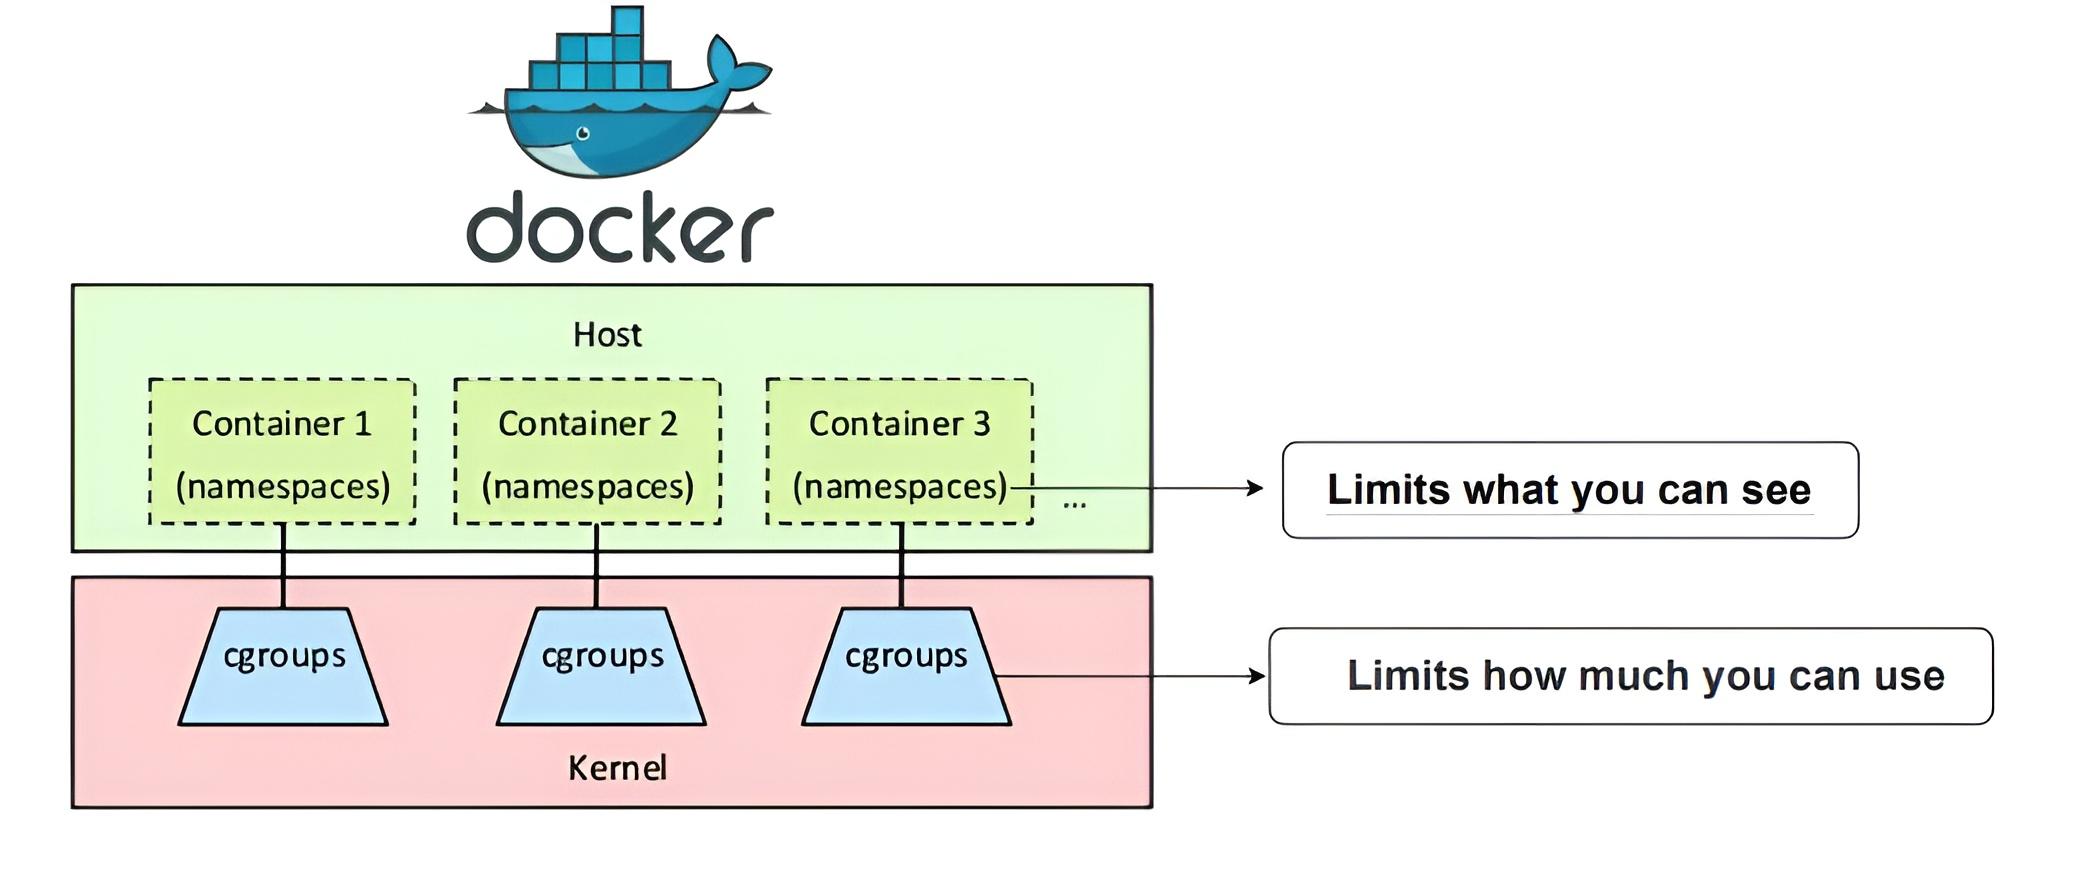
\includegraphics{../images/bikram.jpg}
		}
		\caption{Docker's use of namespaces and cgroups (\cite{dockerbikram})}
	\end{figure}

    Containers are managed by the Docker Container Engine, a daemon (\texttt{dockerd}) which acts as a server, answering the \textit{\acrshort{cli}}'s (\texttt{docker}) \textit{\acrshort{api}} calls. It handles the building, managing, and running of containers, and the download of images (\cite{dockerengine}).
    \linebreak

    However, it's worth noting that Docker wasn't born in a vacuum, nor exists today alone. Several solutions, with similar approach to isolation without virtualization, preceded Docker (one, \textit{\acrshort{lxc}} even being used in it's initial version), and others now compete with it. The \texttt{chroot} command, originally introduced to Unix in 1979, can create ``chroot jails'', that keep programs within that environment from seeing outside of it's root directory. FreeBSD would in 2000 push isolation further by allowing separate configuration and IP addresses in FreeBSD Jails. The next year, Linux VServer added the partitioning of memory. The aforementioned ``cgroups'', were developed in 2006 by Google, and merged to the Linux Kernel (\cite{historycontainers}). \textit{\acrlong{lxc}}, implemented in 2008, was used by Docker (which appeared in 2013) until version 0.9 (2014), when they, while maintaining compatibility, changed to ``libcontainer'', now called ``runC'' (\cite{docker09}). 
    \linebreak
    
    Docker greatly popularized containers with the suite of features their solution had. This popularity resulted in the establishment of the \textit{\acrlong{oci}} by the container industry leaders in 2015 (\cite{aboutoci}). It currently sets three standards: Runtime Specification, Image Specification, and Distribution Specification. These help ensure consistency and interoperability between container related tools and platforms.
    \linebreak
    
    Docker's stack is composed of: the Docker CLI and UI; the Docker Engine (dockerd) that answers them and docker-compose; a high level runtime, containerd, that handles networking and uses runC's API to start and stop containers; containerd-shim to abstract low-level runtimes; and a low-level, OCI compliant container runtime, runC, which actually interacts with the kernel for container operations. The latter is a CLI tool, \texttt{exec}ed in the container's rootfs by containerd. These runC instances cannot outlive their container processes, while containerd can outlive many containers (\cite{journeyfromcontainerization}). Docker donated containerd to the \textit{\acrlong{cncf}} in 2017 (\cite{cncfdocker}), and has since been adopted by other third party low-level runtimes.
    \linebreak

    CoreOS was one of Docker's main competitors, until it was bought by RedHat in 2018. They created several pivotal projects, including rkt, etcd, and Prometheus. They also contributed to Kubernetes. Their low-level container runtime, rkt, competed with runC. However, the project stagnated after the acquisition, and was archived in 2020 (\cite{rktarchived}). 
    \linebreak
    
    RedHat's current alternative to Docker is Podman, a daemon-less container engine in which containers do not need to run with root. Since it is daemon-less, it competes with Docker's containerd and dockerd that, rely on a client-server architecture. Podman's low-level container runtime, equivalent to runC, is ``crun''. Because of both solutions' compliance with OCI, Docker and Podman can be used interchangeably.
    \linebreak

    There are more container runtimes, such as Kata Containers or Firecracker-containerd that offer higher security, aiming for OCI, and containerd compatible sandboxed environments, working for protection closer to VMs. These however have not attracted comparable popularity.





    
    \clearpage
    \subsection{Kubernetes}
    % helm
    Kubernetes is a container orchestrator, with which containerized workloads can be deployed, scaled and managed. Abbreviated as \textit{\acrshort{k8s}}, this platform is often used to host microservice-based implementations. 
    \linebreak
    
    Applications started being deployed to Virtual Machines to keep the resource consumption of each from affecting those of the rest. However, as application deployments started being virtualized, the overhead of each VM's operating system incentivized the move to containers. The resource consumption of containers, and ease of scaling and managing them with Kubernetes feeds directly into the principles and patterns of microservice-based architectures (\cite{k8soverview}). 
    \linebreak

    The platform offers: Service discovery for containers with \textit{\acrshort{dns}} or giving each their own IP and load balancing; Storage system orchestration; Rollouts and rollbacks of deployments, automatically creating and removing containers to match the desired state; ``Self-healing'' by restarting containers that fail; and management of secrets and configuration for the cluster.
    \linebreak

    Kubernetes clusters are groups of one or more nodes (individual machines), with a control plane. The node on which the control plane runs is the cluster's master node, while the rest are worker nodes, onto which pods are deployed depending on their available resources. A pod is the smallest unit of deployment, with one or more containers, that share context (set of Linux namespaces, and cgroups) storage, network and specification. Containers that belong to the same pod all run on the same node (\cite{k8spod}). High-level cluster resources like Deployments, pods, services, replication controllers and secrets can be divided into namespaces, virtual clusters that isolate them from one another. However, resources like nodes or PersistentVolumes are not divided into namespaces (\cite{k8sns}).
    \linebreak

    The control plane is composed of several static pods, that is, pods which aren't managed by a deployment, but defined as static configurations, and run on the master node (\cite{k8sstaticpod}). These components are (\cite{k8scomponents}): 

        \begin{itemize}
            \itemsep0em 
            \item kube-scheduler: monitors etcd through the API server for newly created pods that haven't been assigned a node and selects one for them by available resources, affinities or taints, and constraints.

            \item kube-conrtoller-manager: holds a collection of controllers like the Node controller that reacts to nodes becoming unavailable, or the Job controller that creates pods to run one-off tasks and and follows up on them
            \linebreak
            
            \item kube-apiserver: offers the API which \texttt{kubectl} queries. Clusters can have more than one instance, for horizontal scaling.

            \item etcd: key-value database that backs up the cluster's data, like what container is in which worker node and how long it has been there. It is only accessed directly by kube-apiserver.            
        \end{itemize}

    All nodes, including the master node, run three components: 
        \begin{itemize}
            \itemsep0em 
            \item kubelet: keeps containers in their respective pods, following their specifications, and healthy

            \item kube-proxy: expose the services of the pods in the node
            
            \item Container runtime

        \end{itemize}

    
    \begin{figure}[htb]
		\centering
		\resizebox{.65\linewidth}{!}{%
			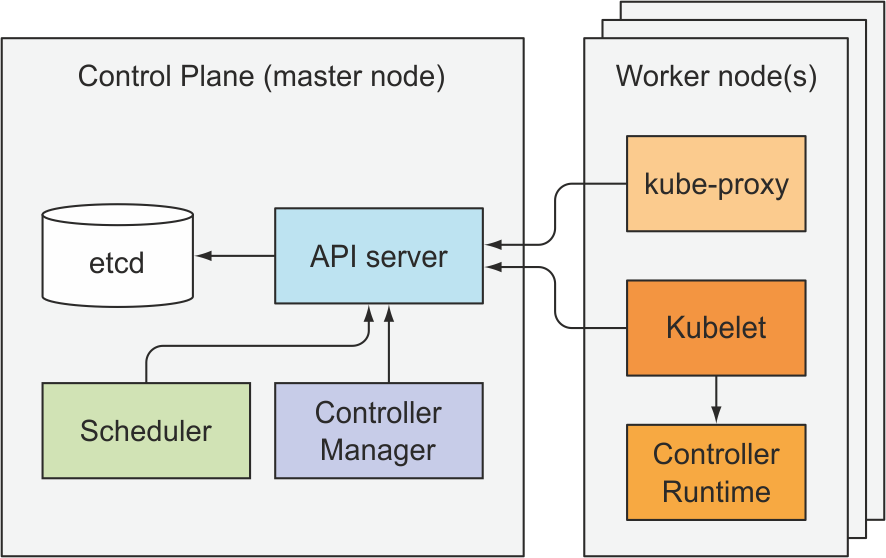
\includegraphics{../images/marko-lukso.png}
		}
		\caption{Kubernetes components of the Control Plane and the worker nodes (\cite{kubernetesmarko})}
	\end{figure}

    Kubernetes can use any container runtime (container engine) that satisfies \textit{\acrshort{cri}} (\textit{\acrlong{cri}}). These include Docker oriented ``dockershim'' and the ``cri-containerd'' plugin, both of which then use containerd to interact with OCI compatible lower-level runtimes (normally Docker's runC); and RedHat's \textit{\acrshort{crio}} (\textit{\acrlong{crio}}), also capable of using OCI compliant runtimes other than Podman's crun (although not supported in OpenShift); among others (\cite{k8scri}).
    \linebreak
    
    Optionally, the features in a cluster can be expanded with Addons, that set up resources in the cluster (normally worker nodes) to offer more functionalities. These can include cluster DNS, ingress, and a dashboard. Deploying source code, and building applications however, are not a part of Kubernetes' responsibilities, instead they fall on CI/CD dedicated tools.
    \linebreak
    
    % Does not deploy source code and does not build your application. Continuous Integration, Delivery, and Deployment (CI/CD) workflows are determined by organization cultures and preferences as well as technical requirements; DAR PASO A DEVOPS

    \clearpage
    \subsection{DevSecOps}
    DevOps is a set of practices, and tools that enable them, to deliver applications and version upon them at a higher velocity, and with improved quality. The goal is to bring together the development and operations teams. Quality assurance and security can also be more tightly incorporated, in what is known as DevSecOps. Methodologies used include continuous integration (frequent merging of code, each validated by automated build and testing processes) for early detection of errors, and continuous delivery or deployment to make changes to the product more rapidly available to the customers. Any code that passes the automated tests is to be considered production ready. The difference between continuous delivery and deployment is the latter takes it one step further, and when changes are pushed to master, these being validated and viable for release, they are automatically deployed to production.
    \linebreak

    DevSecOps integrates security testing into the continuous integration process, having code go through different stages that ensure it's quality. These tests could be run by the developers in their own computers, but there is twofold value to doing them in a pipeline that is common to all. The first is availability, jobs in the pipeline can be run when a commit is made from any machine, regardless of it's capabilities or the software in it. The second is assurance. Having the tests be run on any commit before it's merged means that the automated tests can't be accidentally skipped, and truly ensures that code will have passed the barriers set for it to be considered ready. These tests can be classified in the following:
    \linebreak

        \begin{itemize}
            \itemsep0em 
            \item \textit{\acrlong{sca}} (\textit{\acrshort{sca}}): search for the use of versions of third-party libraries that are known to have vulnerabilities.

            \item \textit{\acrlong{sast}} (\textit{\acrshort{sast}}): identification code smells and potential vulnerabilities in the application's code, and testing, such as unit tests.

            \item \textit{\acrlong{dast}} (\textit{\acrshort{dast}}): looks for security issues during runtime, with simulated attacks like \textit{\acrlong{xss}}, SQL Injections or overlooked endpoints.
            
            \item \textit{\acrlong{cva}} (\textit{\acrshort{cva}}): scanning of Docker images for vulnerabilities in the software they use. It's need can be debated, as although it's useful against public images, if an image comes from a trusted source, or the software in it has already passed SCA and SAST, the step is redundant. For this reason, it's the only one I won't apply in the project.
            
            \item \textit{Infrastructure as Code Security}: ensures the security of infrastructure components that have been defined with code, looking for misconfigurations or issues with compliance that leave security risks.
            

        \end{itemize}
    % several market options are capable of more than one kind of analysis, such as snyk or lacework

    % why cant all steps just be run in the computer of the developer? Are some of these analysis to lengthy, or require the whole application?
    




\clearpage
\section{Cluster setup}
This project's desired end state is a Kubernetes cluster with the elements necessary for DevSecOps, configured and ready, and their readiness demonstrated specifically for \cite{misgit1}. To reach it, I have also chosen to deliver an automated way to do it, that is, a way to repeatably get to the desired state with as little user interaction as possible. The benefits of this approach are two-fold: the process is tracked and reflected, not just in documentation but in the precise list of steps, ready to use; and my effort can be tested and proven without manual interaction for each demonstration, also useful during development.
\linebreak

Achieving this goal calls for shell scripts, Bash in particular, as the tools used benefit greatly from being used in a Linux environment. The project's repository (\cite{misgit2}) holds two scripts which aren't used automatically: \texttt{dns-conf.sh} and \texttt{downloads.sh}. The first configures the host's \texttt{/etc/resolv.conf} and \texttt{etc/NetworkManager/NetworkManager.conf}, both necessary for the cluster's networking at a previous point in development. I currently use \texttt{/etc/hosts} and the cluster's ``coredns'' configmap, but I found value in leaving these remnants for future reference. The second script downloads the binaries for \gls{minikube}, \gls{kubectl} and \gls{helm}, and moves them all to \texttt{/usr/local/bin}. Since the project depends on all three (and more), I also found value in providing a hands-free solution to making them available to my scripts.
\linebreak

The \texttt{launch.sh} is the project's main script, from which all others are triggered in their appropriate order. This script first triggers \texttt{start-cluster.sh}. In it, four main steps are taken: the creation of a \texttt{storage} folder with read, write and execute permissions for all users (some of the configurations for the elements I'll install are accessed by the 1001 user, instead of 1000, which is my own); the creation of a new cluster with three nodes using Minikube; the installation of the Ingress addon in the cluster; and the installation of the Dashboard addon.
\linebreak

Minikube can use different drivers for the nodes, like VirtualBox, but I chose Docker because of the lighter requirements. Also important in the following command, the \texttt{storage} folder is mounted, and will be used to store the cluster's PersistentVolumes.
\linebreak

    \begin{figure}[htb]
        \centering
        \begin{subfigure}{.7\textwidth}
            \hspace{-5cm}
            \inputminted[fontsize=\scriptsize, firstline=60, lastline=62, linenos, frame=single, tabsize=1]{bash}{../../start-cluster.sh}
          \end{subfigure}
        \caption{Minikube create cluster, \texttt{start-cluster.sh} (O. Salvador, 2023)}
    \end{figure}
    \linebreak

\clearpage
After enabling the Dashboard addon, a web UI is made available in localhost, although the port changes with each execution. Within it, the now created nodes can be seen.

    \begin{figure}[htb]
		\centering
		\resizebox{.8\linewidth}{!}{%
			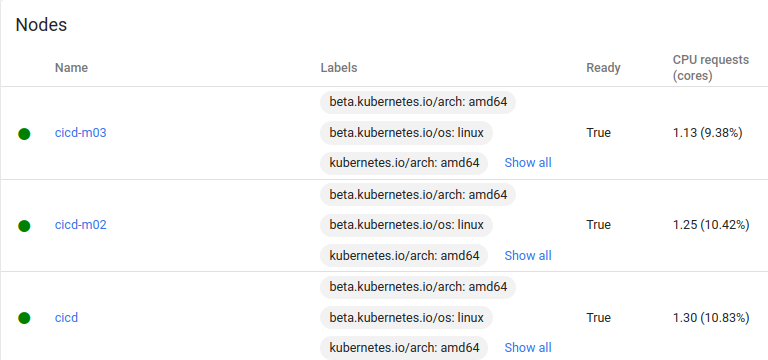
\includegraphics{../images/cluster_allnodes2.png}
		}
		\caption{Dashboard view of the nodes in the cluster (\cite{kubernetesmarko})}
	\end{figure}

The other mentioned addon, Ingress, is one of the ways with which the services in a cluster can be accessed from the outside, and the one I've chose for this project because of it's simplicity. While there are alternatives, the default ingress addon uses an NGINX server. Outside access is most often HTTP or HTTPS. Since this report has DevSecOps in it's name, I believe that implies an obligation to use the latter. Therefore, I create my own certificates.
\linebreak

Kubernetes offers it's own default certificate, but because it's generated by the Kubernetes ingress controller (issued by the same system that created it, self-signed) and not signed by a trusted \textit{\acrshort{ca}} (\textit{\acrlong{ca}}, it isn't valid. To solve this I created the \texttt{certificates.sh} script in \texttt{gitlab/configure}, although it isn't triggered at this point. It uses \texttt{easy-rsa} (\cite{easyrsadocs}), that helps manage X.509 \textit{\acrshort{pki}}. With it, the script creates a new PKI and CA (that I've named ``CA Ltd''). Once the CA is created, a new private key is generated using \texttt{openssl}. This key is then used in a \textit{\acrshort{csr}} (\textit{\acrlong{csr}}) which's fields are automatically filled by feeding the text lines with \texttt{EOF}. A new key is needed for each new certificate. The CSR is sent to the PKI to be signed. With the CSR signed, a certificate for the domain can be created. 
\linebreak

The last two things the script does is load the certificate to the host and then to the cluster. First it copies the script to \texttt{/usr/share/ca-certificates/trust-source/anchors}, and then creates a \textit{\acrshort{tls}} secret in the gitlab namespace with the certificate and it's private key. Another secret is also created, holding the private key. For the ingress controller to use the newly created certificate secret, it's deployment needs to be restarted. Now, when a request is made to GitLab using HTTPS, the ingress controller will perform a TLS handshake, in it, the client and server exchange certificates and a secure connection gets established. Because the certificate is no longer singed by the same system that is using it, and I've set the CA as trusted in the client's host, the client will consider it valid, and proceed with the encrypted communication (\cite{badawy}).
\linebreak


    \begin{figure}[htb]
		\centering
		\resizebox{.9\linewidth}{!}{%
			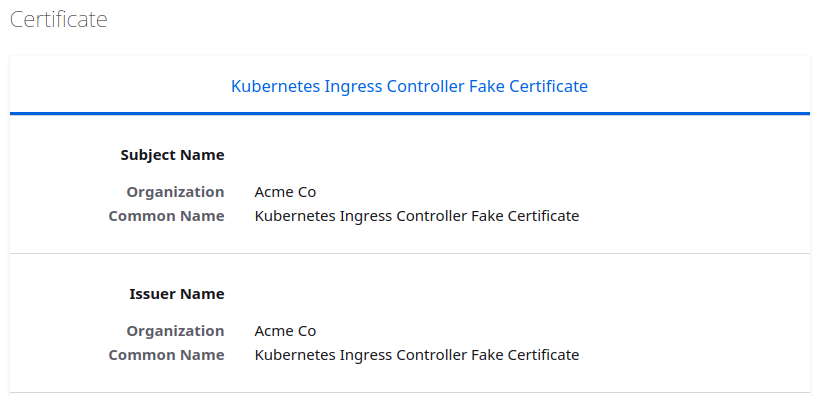
\includegraphics{../images/cert-k8s.png}
		}
		\caption{Kubernetes self-signed certificate (O. Salvador, 2023)}
	\end{figure}

    \bigskip
    
    \begin{figure}[htb]
		\centering
		\resizebox{.9\linewidth}{!}{%
			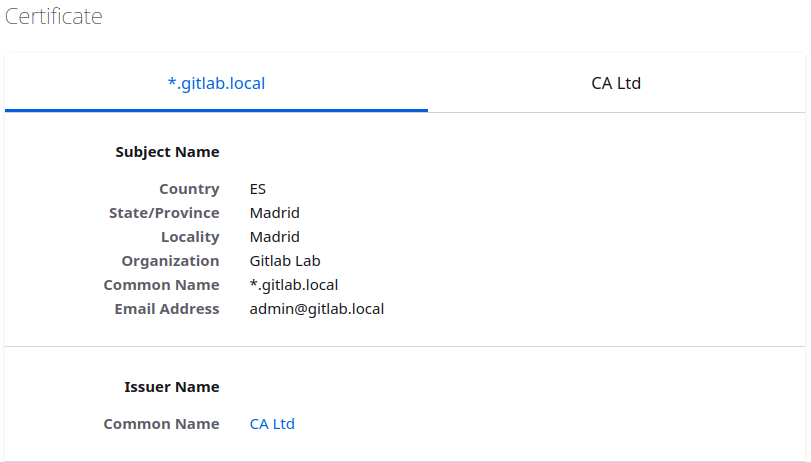
\includegraphics{../images/cert-mio.png}
		}
		\caption{Certificate created by \texttt{certificates.sh} (O. Salvador, 2023)}
	\end{figure}

 
 
    
    \clearpage
    \subsection{GitLab}
    GitLab is an open-source and self-hostable DevOps solution, that offers a complete platform, with repositories, issue-tracking, wikis, pipelines and artifact storage for each project. The possibility to host it locally for free (with the Community Edition) and my previous experience with it, during my summer internship at TechSociety made it a great candidate. Additionally, the comprehensive set of features led me to choose it over more minimalist solutions, like Gitea or Gogs which don't offer built-in pipelines or artifact storage, and would have required the installation of dedicated solutions, like Jenkins and Artifactory. 
    \linebreak

    Once the cluster is already started, and the dashboard is accessible, the \texttt{launch.sh} script triggers \texttt{gitlab/gitlab-helm.sh}. This script first reads \texttt{/etc/hosts} to check if there is an entry with the cluster's IP address and the subdomains hanging from ``gitlab.local'' that'll be used later on, and appends it if there isn't. It's important to take this step before the next, because during the installation, pods will search for the services of each other, with those subdomains, and fail if they can't find them. This was the case before I started using Ingress.
    \linebreak

    Before installing the GitLab Helm chart, I create a dedicated namespace and switch to it. Once in it, I also apply \texttt{gitlab/pvc-locales.yml}, a YAML file in which I describe the PersistentVolumes and PersistentVolumeClaims for gitlab, configuring their ``accessModes'' to ``ReadWriteOnce'' and ``volumeName''. I found this step necessary for the cluster to be able to read those PersistentVolumes after being paused, stopped and started again, and for the pods to be able to find their storage when the cluster has more than one node. Lastly, before installing GitLab, it's at this point that the \texttt{gitlab/configure/certificates.sh} script is run, creating the certificate and storing it as a secret in this namespace.
    \linebreak

    GitLab's default Helm chart had difficulties reliably finding the PersistentVolumes it creates, failing the installation, and also reading from them after restarting the cluster. This led me to use another YAML, \texttt{gitlab/values2.yml}, picking the options I wished to overwrite from the default from the list of examples in the chart's repository (\cite{gitlabchart}). In it, I configure the ``secretName'' under which I uploaded the certificate, the domain, the use of HTTPS, and the settings for persistence among others. The gitlab-runner's ``certSecretName'' is also specified in this file, so that the runner will find it and properly connect with the server. The multiple ``volumeName'' sub-fields in this YAML match the ones in the previous YAML, in which the PVs and PVCs were declared. 
    \linebreak

        \begin{figure}[htb]
            \centering
            \begin{subfigure}{.7\textwidth}
                \hspace{-5cm}
                \inputminted[fontsize=\scriptsize, firstline=2, lastline=2, linenos, frame=single, tabsize=1]{bash}{../../gitlab/values2.yml}
                \vspace{-.5cm}
                \inputminted[fontsize=\scriptsize, firstline=8, lastline=16, linenos, frame=single, tabsize=1]{bash}{../../gitlab/values2.yml}
                \vspace{-.6cm}
                \inputminted[fontsize=\scriptsize, firstline=25, lastline=28, linenos, frame=single, tabsize=1]{bash}{../../gitlab/values2.yml}
              \end{subfigure}
            \caption{Domain and secrets in \texttt{gitlab/values2.yml} (O. Salvador, 2023)}
        \end{figure}

    The only value that isn't in \texttt{gitlab/values2.yml} is the cluster's IP, since it changes with each host, and I want this set of scripts to work on other people's machines with as little tinkering needed as possible. 
    \linebreak
    
        \begin{figure}[htb]
            \centering
            \begin{subfigure}{.7\textwidth}
                \hspace{-5cm}
                \inputminted[fontsize=\scriptsize, firstline=31, lastline=32, linenos, frame=single, tabsize=1]{bash}{../../gitlab/gitlab-helm.sh}
              \end{subfigure}
            \caption{Helm command to install the GitLab chart, \texttt{gitlab/gitlab-helm.sh} (O. Salvador, 2023)}
        \end{figure}

    Installing the chart onto the cluster doesn't mean it's services will be immediately available. While the elements in the namespace are being set up, the script enters a loop waiting until six folders in \texttt{storage} have been created, all with 777 permissions, giving said permissions to all folders within it and sleeping for ten seconds with each iteration. Knowing of PostgreSQL's use of the 1001 user due to previous experience, and of it being used by GitLab from reading it's chart's template, is the main reason for which I started doing this, but giving this treatment to all ensures none will fail over it. 
    \linebreak
    
    Once this wait is over, we can be confident all PersistentVolumes will have the permissions they need. After this, the script enters a second \textit{while} loop, querying the ``\texttt{users/sign\_in}'' endpoint at my GitLab installation's domain until it returns a status code of 200, or a failure in the resolution of the webservice with a code in the four hundreds. The use of this endpoint is important, since it's the only one from which queries will not be redirected, and thus cURL will not return 308 as a result.
    \linebreak
            
    While not executed right after \texttt{gitlab/gitlab-helm.sh}, the script \texttt{personal-access-token.sh} in \texttt{gitlab/configure} could be run the moment the former finishes. My reason not to is grouping, I chose to run it later, right before it's actually needed. Unlike the other scripts, this one is run with \texttt{source}, so that the variables in it are available to the rest of the commands and scripts in \texttt{launch.sh}. The one that is used, and which gives the script it's name, is the Admin's \texttt{\$PERSONAL\_ACCESS\_TOKEN}, necessary for most interactions with GitLab's API. It cant' however just be created from the Admin's username and password, the former always ``root'', and the value of latter held in the secret ``gitlab-gitlab-initial-root-password'' in the namespace, that I retrieve and decode from base64. 
    \linebreak
    
    With these credentials, an ``oauth token'' must first be created (\cite{gitlabpat}, \cite{gitlabpatusers}). This token can then be used to query the API to create a \textit{\acrshort{pat}} for the Admin. I create it with access to all scopes, and an expiration date two weeks after the command is run. Full access is required for the uses it will fulfill.
    \linebreak
        %\inputminted[fontsize=\scriptsize, firstline=10, lastline=18, linenos, frame=single, tabsize=1, breaklines, breakafter=/, breakaftersymbolpre={}]{bash}{../../gitlab/configure/personal-access-token.sh}
        
    The script that \texttt{launch.sh} does get triggered after \texttt{gitlab/gitlab-helm.sh} is \texttt{coredns.sh}. This script gets the JSON with the details of the ``coredns'' configmap of the ``kube-system'' (default in all Kubernetes clusters) and appends to it a new domain, ``gitlab.local'' under which several subdomains are mapped to the hostIP of the ``ingress-nginx-controller'' from the ``ingress-nginx'' namespace. The most important subdomain is Sonarqube's, it's full domain being \texttt{sonarqube.gitlab.local} in my case, although configurable for different base domains. This modification is important, as without it, Sonarqube will not be accessible from within the cluster. 
    \linebreak

        \begin{figure}[htb]
            \centering
            \begin{subfigure}{.7\textwidth}
                \hspace{-5cm}
                \inputminted[fontsize=\scriptsize, firstline=5, lastline=12, linenos, frame=single, tabsize=1, breaklines]{bash}{../../coredns.sh}
              \end{subfigure}
            \caption{Extract to be appended to coredns, \texttt{coredns.sh} (O. Salvador, 2023)}
        \end{figure}
    

    
    \clearpage
    \subsection{Sonarqube}
    Sonarqube is a self-hostable tool that can scan source code to inform of code quality issues, such as: code smells, bugs, or lack of unit testing coverage. It can be integrated into CI pipelines like the ones I want to use in GitLab, and offers Gates, thresholds of minimum quality to meet before the job in which Sonarqube is run succeeds. This is valuable, as it allows code, which might or might not have passed SAST in the computer of whoever is trying to make a commit, to have go through it before the changes are accepted.
    \linebreak

    Unlike the rest of analysis tools that'll be used in pipelines, Sonarqube needs to be installed in the cluster to be available in them. This is because, while they distribute a Sonarqube docker image, it's just a client, that needs to connect to a server. It's this server and the database that it requires which make it necessary to install the Sonarqube chart in the cluster. 
    \linebreak
    
    \begin{figure}[htb]
		\centering
		\resizebox{\linewidth}{!}{%
			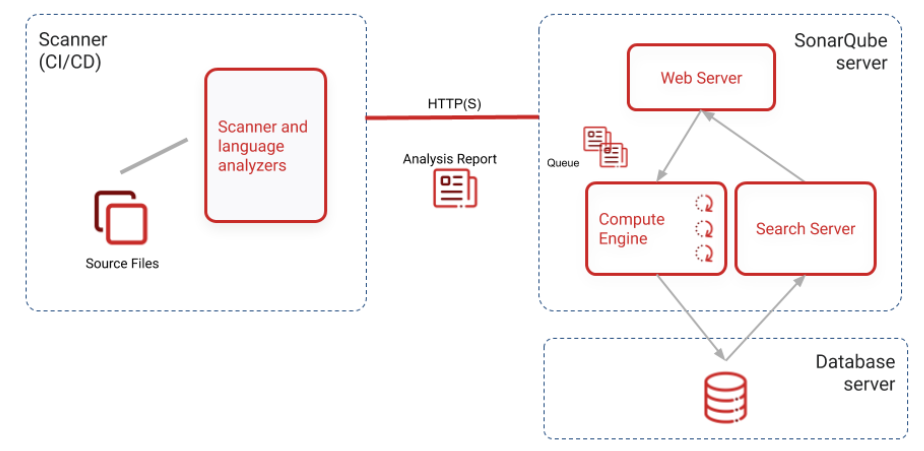
\includegraphics{../images/sonarqube.png}
		}
		\caption{Sonarqube instance components (\cite{sonarqubeinstall})}
	\end{figure}

    Sonarqube can use one of multiple external database engines, having support for Microsoft SQL Server, Oracle and PostgreSQL (\cite{sonarqubeinstall})). By default, the chart uses PostgreSQL. Since this database engine is open source and free to use, it's the most interesting to me. As before, since it'll be accessed by the user 1001, in the script \texttt{sonarqube/sonarqube-helm.sh}, after creating the namespace for sonarqube and switching to it in kubectl's context, I create two new folders in \texttt{storage} and make sure they have 777 permissions, for the server and database. With those taken care of, the two PersistentVolumes in \texttt{sonarqube/pv-sonarqube.yml} can be created, under the names Sonarqube's chart is expecting.
    \linebreak

    Once the PersistentVolumes Sonarqube expects have been fixed, the script uses Helm to install Bitnami's (verified third party that packages applications and offers Helm charts and Docker images) Sonarqube chart setting it's service to ``NodePort''. By configuring it here, and having modified the ``coredns'' configmap, the service described in \texttt{sonarqube/svc-sonarqube.yml} no longer needs to be applied for Sonarqube to be discover-able within the cluster.
    \linebreak

    However, for it to be accessible from the outside, and ingress also needs to be applied. This is described in \texttt{sonarqube/ing-sonarqube.yml}. In this YAML, the name of the secret with the TLS certificate is also specified, in the same way as it was for GitLab. The secret has both the same name and contents as it did there as well, but because this is a separate namespace, has to be created just before the Ingress is applied. With it applied, Sonarqube has everything needs, and after a short while (both the physical wait and the loop that is used to keep the script from progressing, as I did in GitLab's script), it's webservice will be accessible through HTTPS at the subdomain \texttt{sonarqube} under \texttt{gitlab.local}. 
    \linebreak

    When the webservice becomes available, \texttt{launch.sh} continues, the next thing it does being the launch of a query to Sonarqube's API. The query uses Sonarqube's initial user credentials, ``user'' as username and a six-digit randomly generated string as password. The latter can be retrieved from the cluster, where it's kept as a secret under the name ``sonar-sonarqube''. With these, the API authenticates, and since these credentials are for the Administrator, authorizes the query. This one asks for the creation of a user token, which will be necessary in the pipelines. It is therefore stored as an environment variable for use later on in \texttt{launch.sh}'s runtime. This value and other useful ones of the execution, like GitLab's token (which is created just after this one), are stored in \texttt{/tmp/cluster.txt}, a disposable file with values the script uses, and that helped me during debug, as I executed it's commands \textit{\gls{adhoc}}.
    \linebreak
    
        \begin{figure}[htb]
            \centering
            \begin{subfigure}{.8\textwidth}
                \hspace{-5cm}
                \inputminted[fontsize=\scriptsize, firstline=15, lastline=17, linenos, frame=single, tabsize=1, breaklines]{bash}{../../launch.sh}
              \end{subfigure}
            \caption{Creation of the Sonarqube user token, \texttt{launch.sh} (O. Salvador, 2023)}
        \end{figure}


    
    \clearpage
    \subsection{Runner setup}
    GitLab runners are daemons, long lasting programs, that wait for the GitLab instance to send jobs from pipelines that have to be executed their way, and return the results. Runners can be configured so that any project can run it's jobs on it, being ``shared'', limited to the projects in a group, or specific to a single project. They can also be tagged, so that jobs with matching tags seek them out. This is is useful to signal specific available software
    \linebreak

    After creating the tokens for Sonarqube and GitLab, \texttt{launch.sh} triggers \texttt{gitlab/configure/generate-runner-setup.sh}. This script is basically an echo with another script inside, that gets redirected to a new script, \texttt{runner-setup.sh} with values that change on each setup of the cluster. Into this script, it's parent copies the contents of the certificate, as text, so that the child, when executed, prints them to a file, and copies this file into the \texttt{/usr/share/ca-certificates/trust-source/anchors} folder of whichever machine \texttt{runner-setup.sh} is executed in. This ensures that, if the target machine has access to the cluster, it'll be able to use HTTPS. The script then downloads the gitlab-runner program, a binary. The script gives it permissions and launches it, setting up a runner in the machine authenticating with the Admin PAT. I run this script on a virtual machine, with Azure CLI (already logged into) and Docker (for building images). Multiple runners can be registered from a host.
    \linebreak
    
        \begin{figure}[htb]
    		\centering
    		\resizebox{.95\linewidth}{!}{%
    			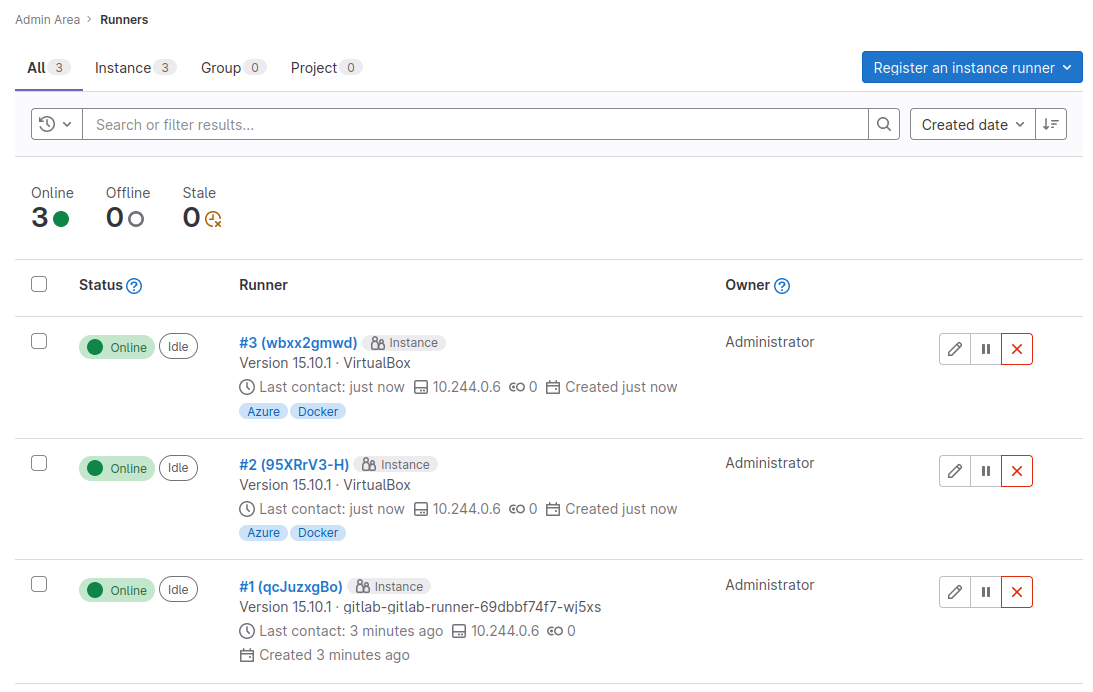
\includegraphics{../images/gitlab-one-vm-two-runners.png}
    		}
    		\caption{Two runners from the same host registered in GitLab (O. Salvador, 2023)}
    	\end{figure}


    \clearpage
    \subsection{GitLab configuration}
    GitLab's instance comes nearly empty, with just a default project. In GitLab, a project contains a repository, it's single pipeline (with no differenciation between CI and CD), project variables, wiki, kanban and project settings. At this point in the \texttt{launch.sh} script, it could be stopped and a different application, or set of them, configured to use the instance. Since this report aims to setup a demonstration of DevSecOps with the application developed for the previous report, several resources within the instance need to be provisioned to accommodate it. Because there are many, using GitLab's API would quickly become tedious. As I have experience with Terraform, I've chose to use it to configure GitLab, having \texttt{launch.sh} apply a Terraform project that provisions these resources. To develop it, I used the official Terraform documentation for the GitLab provider (\cite{gitlabprovider}). During the initial configuration, \cite{seppanen} helped me find how to specify the use of a custom instance, instead of the official GitLab site (use of the \texttt{base\_url} variable).
    \linebreak
    
    The first resources are groups, within which to organize projects. I have described two to be created. One for repositories dedicated to infrastructure as code (infrastructure-repos), the Terraform projects that deploy the application's required SaaS resources to Azure, and another for the source code of the fullstack application's components (backend and frontend servers). In my previous report I developed the IaC for the project in both Terraform and Ansible, but since more IaC security tools are available for Terraform, and because each would require their own GitLab projects and pipelines (tailored to them), I have chosen to just work with the Terraform set. 
    \linebreak
    
        \begin{figure}[htb]
    		\centering
    		\resizebox{.95\linewidth}{!}{%
    			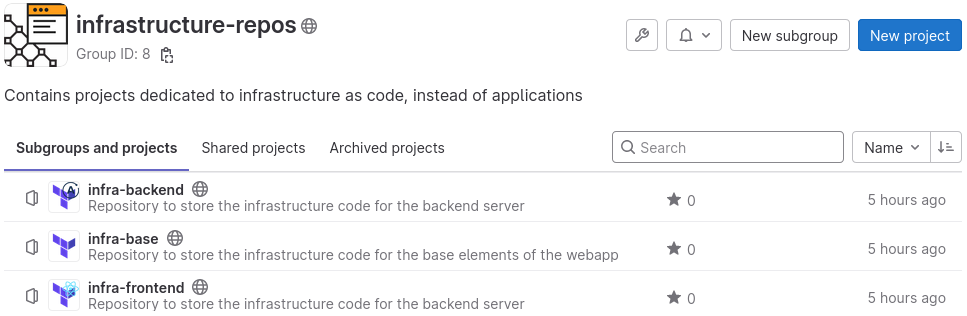
\includegraphics{../images/infrarepos.png}
    		}
    		\caption{IaC group with three GitLab projects (O. Salvador, 2023)}
    	\end{figure}
     
    Three different Terraform projects are used, one for the first wave of components that needs to be created, with resources such as the Virtual Net, and Databases (Redis and CosmoDB), another for the Azure Container Instance in which the backend's Docker image will run, and another one for the frontend's image. This separation, necessary to accommodate for the ACI's need of an image that first has to be build and pushed to an ACR that itself needs to be provisioned, has the benefit of greater decoupling, of both the development and deployment of the infrastructure described in their code.
    \linebreak


        \begin{figure}[htb]
    		\centering
    		\resizebox{.95\linewidth}{!}{%
    			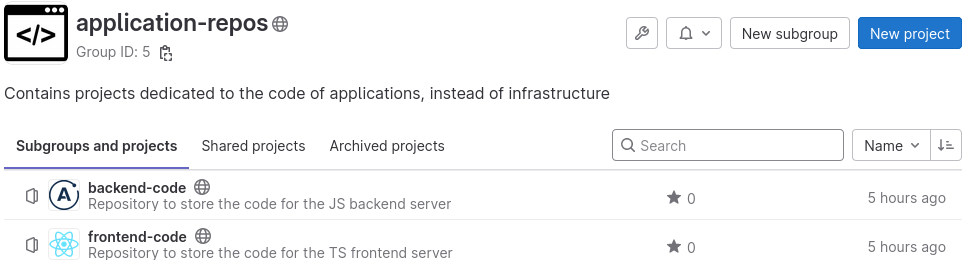
\includegraphics{../images/aplicationrepos.png}
    		}
    		\caption{Source code group with two GitLab projects (O. Salvador, 2023)}
    	\end{figure}

    Within each GitLab project, two execution environments are created. Environments are specific to each project, they can't be created at a higher level, like their groups, or a root group. They allow for different sets of execution variables, and a logical separation of the pipelines and jobs that run in each environment. The same two environments are created for all projects, ``production'' and ``preproduction''. Since this is just a small-scale demonstrator, I have merged into preproduction what would normally be two environments: ``develop'' and ``staging'' (also called \textit{\acrshort{uat}}). The reason for this simplification is cost, since each environment will have it's own set of resources in Azure, and these are billed for, yet a third environment provides little additional insight.
    \linebreak

    GitLab variables can be configured at the group or project level, and limited to specific environments within the projects that inherit them. This way, jobs can consume different values, offering different results depending on the environment in which they are executed. They way I've set them in the GitLab configuring Terraform project, variables that hold the same value in every environment (in my case the Azure subscription and location for the resources among others) are available to all using a wildcard. Values like the Azure resource group names (one for production and another for preproduction) or the names of the resources in them, are set as specific to their corresponding environment. Depending on the branch of the infrastructure project that is being deployed, Terraform will create resources in one resource group or the other, prefixing the resources in preproduction with ``pre'' in their names. Names, values and settings for most variables are taken from the \texttt{variables.tfvars} variable file in the Terraform project that configures GitLab. However, there are two variables which are not: ``\texttt{SONAR\_TOKEN}'' and ``\texttt{SONAR\_KEYSTORE\_PW}'' these will be used to interact with Sonarqube by the pipelines of the projects that hold application source code.
    \linebreak

    The last resources described in this Terraform project are GitLab users, repository branch protections, and project memberships. Projects do not need to have their repository initialized to be configured, or branches (even if they don't yet exist) protected. As with all resources in the Terraform project but the two aforementioned variables, GitLab projects are described as objects in a list in \texttt{variables.tfvars}, and the attributes of each object used in the HCL code to provision the resources. GitLab projects are listed with the members I want each project to have, and their kind of access. Memberships are the type of relationship a GitLab user holds with a project, categorized by permissions into roles (Developer, Maintainer, Owner). 
    \linebreak
    
    Three users are created, their creative names descriptive of the access they are to have: ``developer1'', ``developer2'' and ``maintainer1''. Code projects list the developers and maintainer as their members, while IaC projects only give access of any kind to the maintainer.
    \linebreak
    
        \begin{figure}[htb]
    		\centering
    		\resizebox{.6\linewidth}{!}{%
    			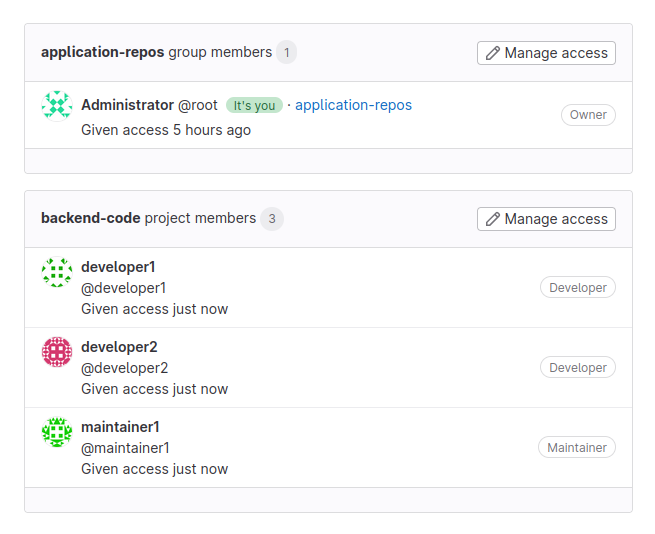
\includegraphics{../images/gitlab-project-members.png}
    		}
    		\caption{Members of \texttt{backend-code} and their access level (O. Salvador, 2023)}
    	\end{figure}

    Code projects get protections to the branches ``master'' and ``develop'', prohibiting the direct push of commits to just the maintainer, but giving merge access to the developers. Infrastructure projects only allow access of either kind to the maintainer. I originally considered outright barring any direct push to either, to force the need to merge from ephemeral feature branches to develop, and from develop to master. Eventually I opted against it in consideration of hot-fixes, so that not just the Administrator (who has Owner access to all branches in all projects) can make a quick change in case of emergency. Once the resources in GitLab have been provisioned and configured, code can be committed to the newly created projects. This is done by the \texttt{setup-repos.sh} script in \texttt{gitlab/configure}, the last script to be triggered by \texttt{launch.sh}.
    \linebreak

    This script first creates a truststore with the certificate. This truststore is the only way for the Sonarqube scanner (the client that runs in pipelines and connects with the server) to have access to the certificate, without which HTTPS communication is impossible, and it won't trust the server.

        \begin{figure}[htb]
            \centering
            \begin{subfigure}{.8\textwidth}
                \hspace{-5cm}
                \inputminted[fontsize=\scriptsize, firstline=134, lastline=135, linenos, frame=single, tabsize=1, breaklines]{bash}{../../gitlab/configure/setup-repos.sh}
              \end{subfigure}
            \caption{Truststore creation with keytool \texttt{setup\_repos.sh} (O. Salvador, 2023)}
        \end{figure}
    
% mencionar los ficheros seguros
    The script then clones \cite{misgit1}, and copies the file to the backend and frontend folders. These will be uploaded into their respective repositories, and so, the truststore will be available as another file in them, that will be possible to use in the pipelines. GitLab is in the process of developing encrypted project files (\cite{securefilesapi}), these are like project variables, not part of the repository but rather to be used in pipelines. However, at the time I was developing this project, the tool that's to be used to access them (\cite{downloadsecurefiles}) needs the certificate to be available to it. Since I would have used it to upload the certificate, using it would have been redundant, and uploading it in an encrypted truststore was the better option. On each of the original repository's folders (backend, frontend and the three original Terraform projects), the script runs the function \texttt{repo\_surgeon()}. This initializes a new git repository locally and creates two branches in each. For IaC repositories, these are production and preproduction, while code repositories get master and develop. For each branch of each repository, the script copies the corresponding pipeline YAML (from \texttt{gitlab/configure/pipelines} to them as \texttt{gitlab-ci.yml}, and pushes a commit with the changes to their GitLab project.
    \linebreak

    Another function, \texttt{start\_jobs()} is also present in the script, but all calls to it have been commented before this report's delivery. The function reads Terraform's output, that I've set to hold the names and ids of the projects created by Terraform, as a JSON. Upon being called, the function uses \texttt{jq} to parse the JSON and retrieve the id of a project from it's name, which it receives as a parameter. With it, four different queries are made. The first retrieves the list of jobs from the project that are currently running, and is repeated in a loop until none are left. The next query finds any manual jobs, which won't have been triggered. These are looped over, starting them with the third. The last query is then made, in another loop, waiting until the newly started jobs are no longer running. This function was useful during development, automatically triggering all the jobs from pipelines across all projects, in the order they need to be started. It is not necessary during normal operation, as I intend the pipelines to be triggered independently by their users as needed, without unnecessary dependencies.





    

\clearpage
\section{Pipelines}
The complete system, once \texttt{launch.sh} has successfully finished it's execution, has a Kubernetes cluster with Sonarqube and GitLab installed in it, HTTPS communication setup all throughout, a runner on another host (that needs to have visibility of the cluster), and GitLab projects for the webapp configured, with branches, branch protections, variables, separate environments for production and preproduction, and pipelines to provision it's infrastructure and deploy it's code.
\linebreak

    \begin{figure}[htb]
        \centering
        \resizebox{\linewidth}{!}{%
            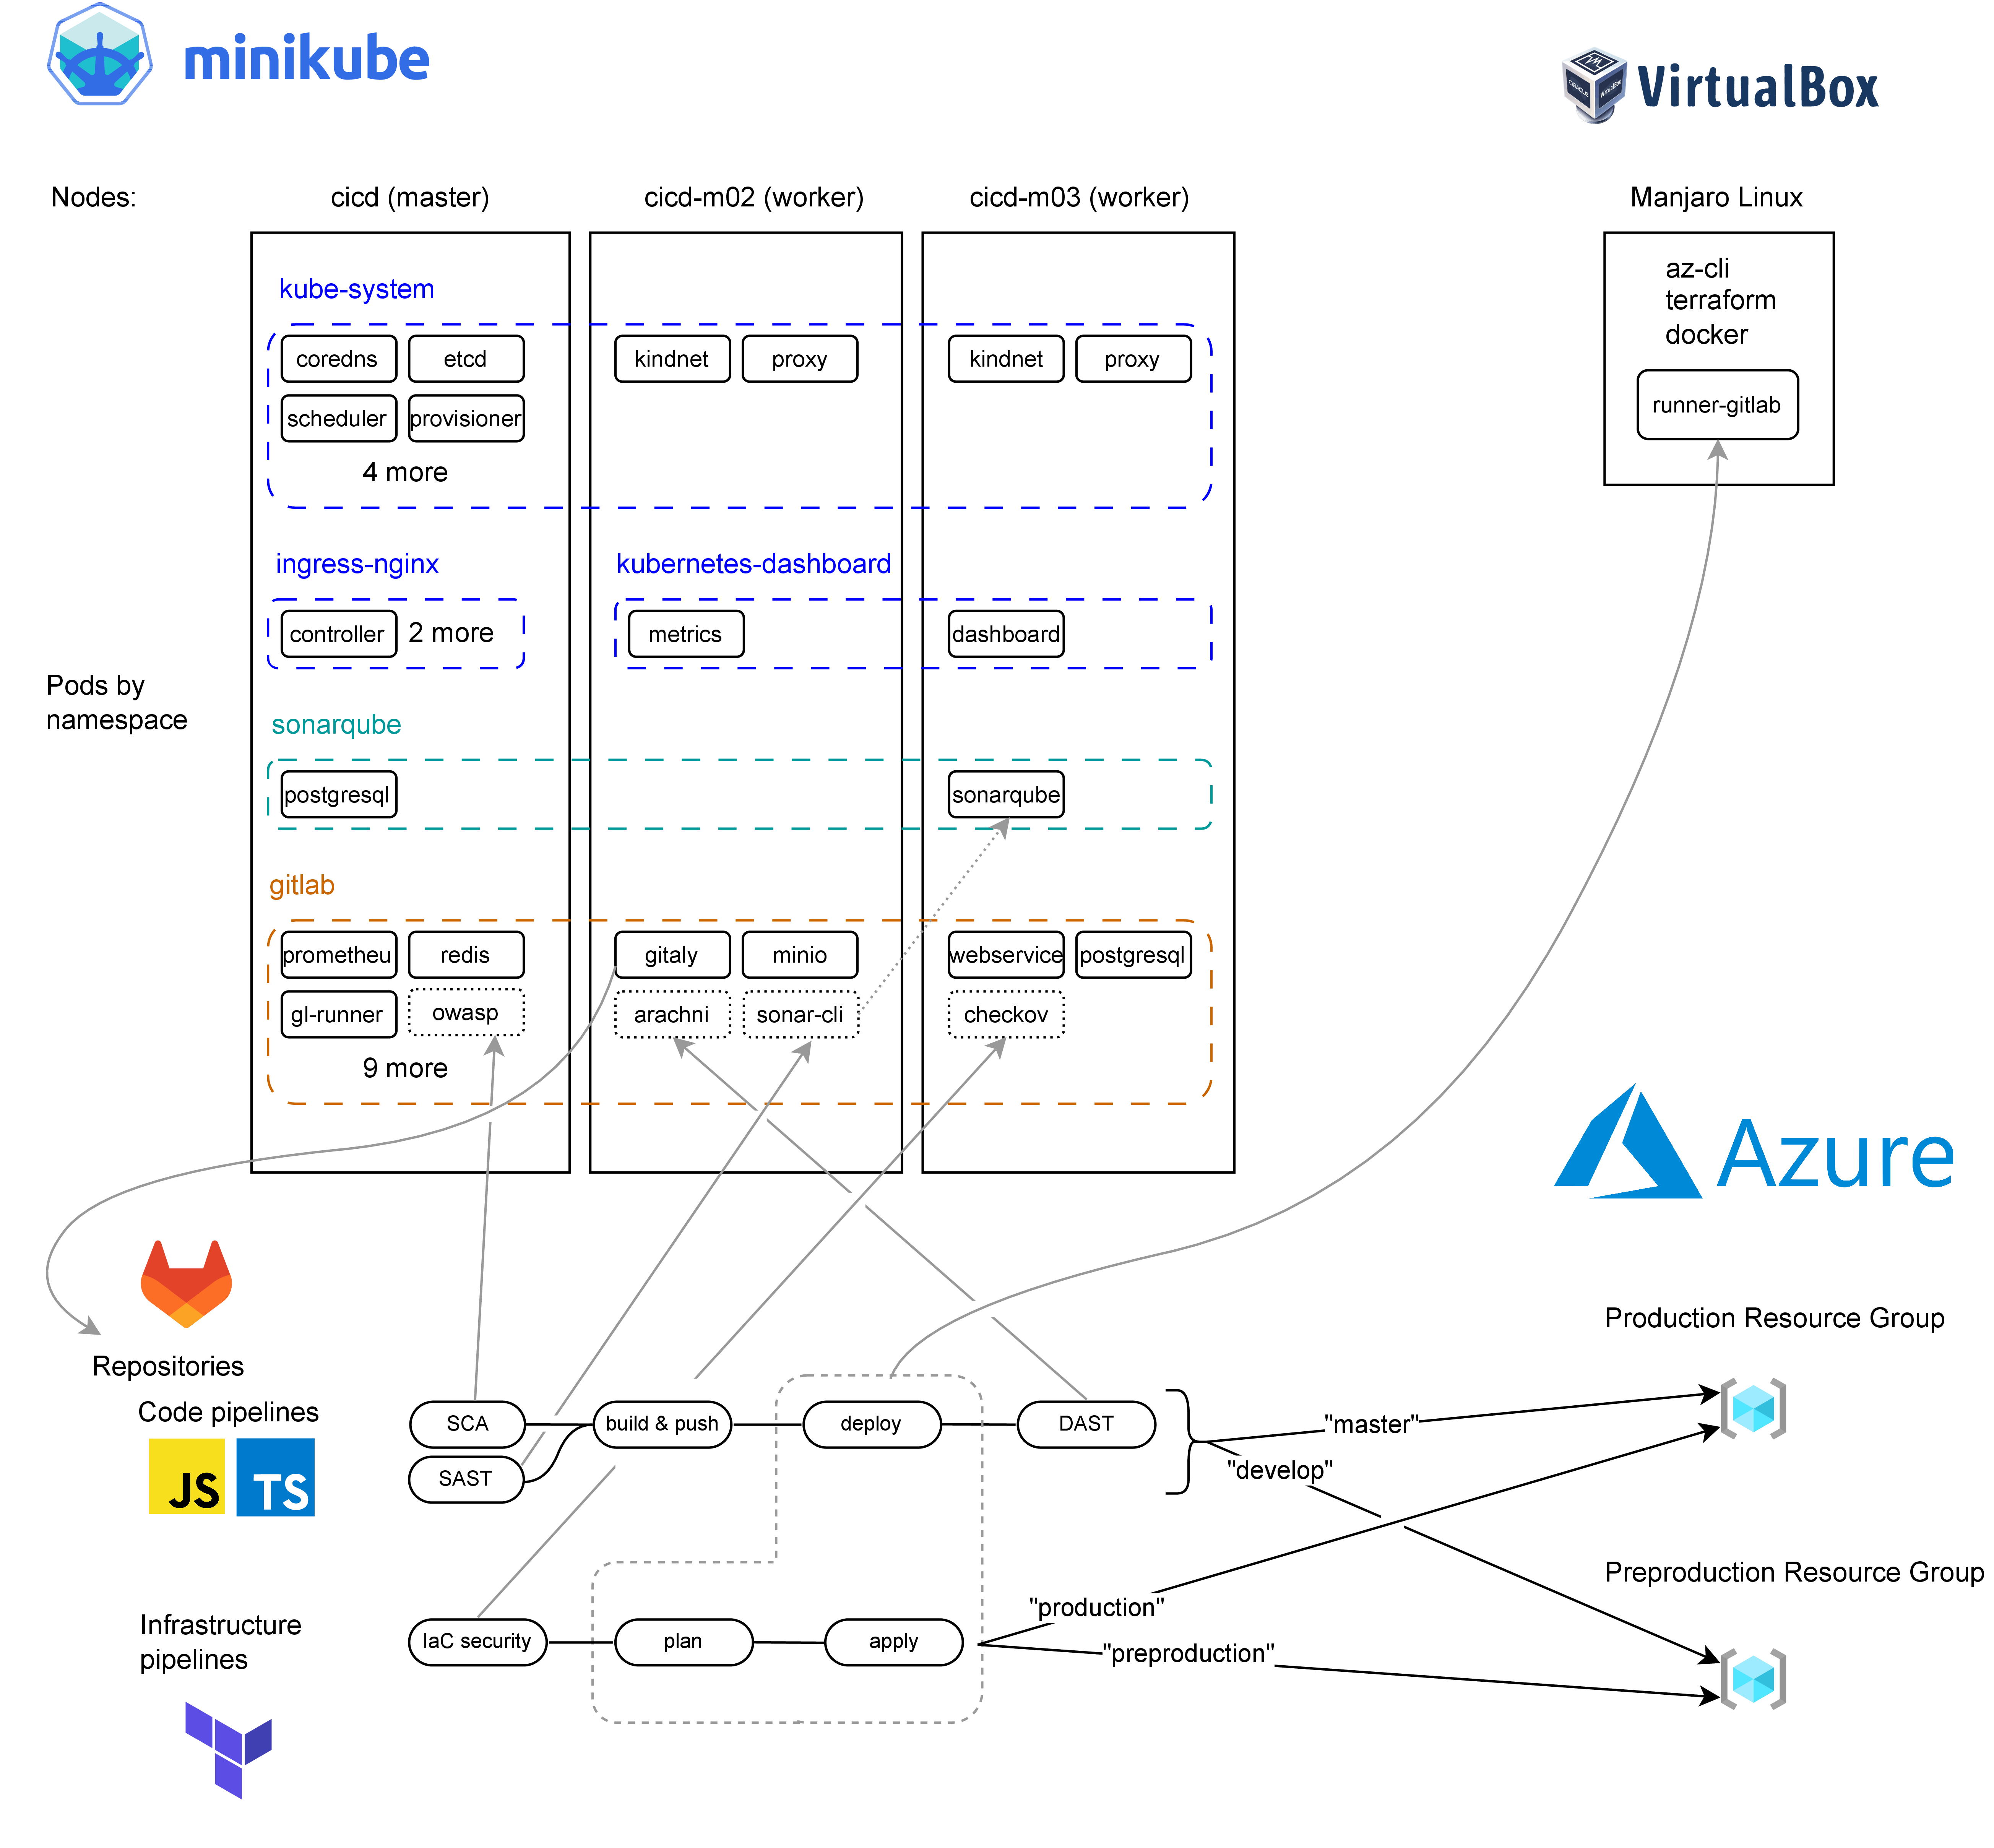
\includegraphics{../images/cluster2.drawio.png}
        }
        \caption{ (O. Salvador, 2023)}
    \end{figure}

The same pipelines are used in all infrastructure projects, one for preproduction and another for production. The only difference between them is the environment they use. In some cases, it's desirable to have the same system for both, with ``dev'' and ``UAT'' being functional mirrors of ``pro''. Other times, it's best to have a simplified system, specially for development to save on costs, even if UAT is indeed similar to production. In this one, the environments are identical, since I found no resources that could be removed while keeping the system functional. Because I use the same two YAMLs (pro and pre) for all projects, I only have one copy of each, with soft links making them appear replicated under the names of ``infra-base'', ``infra-backend'' and ``infra-frontend''. They have three stages:
\linebreak

Pipelines for code projects are different among them, but shared among their branches. Unlike the IaC projects, production and preproduction in code projects are meant to be merged together at given points, instead of permanently drifting apart. The same pipeline is used for the backend's master and develop, and a different YAML used in the frontend, but also by both of it's branches.
\linebreak

    \bigskip
    \bigskip
    \subsection{Infrastructure pipelines}
    The three stages in infrastructure pipelines are:
        \begin{itemize}
            \itemsep0em 
            \item IaC security scan with Checkov (it's free to use and open source)
    
            \item Terraform plan with the appropriate environment variables in the runner that has \texttt{terraform} and \texttt{az-cli} installed and logged into
            
            \item Terraform apply, in the same conditions as plan, but only executed manually    
        \end{itemize}

    Checkov reads the HCL files in which the resources to provision are described, and looks for misconfigurations or anti-patterns that could be exploited.
    
        \begin{figure}[htb]
            \centering
            \resizebox{.75\linewidth}{!}{%
                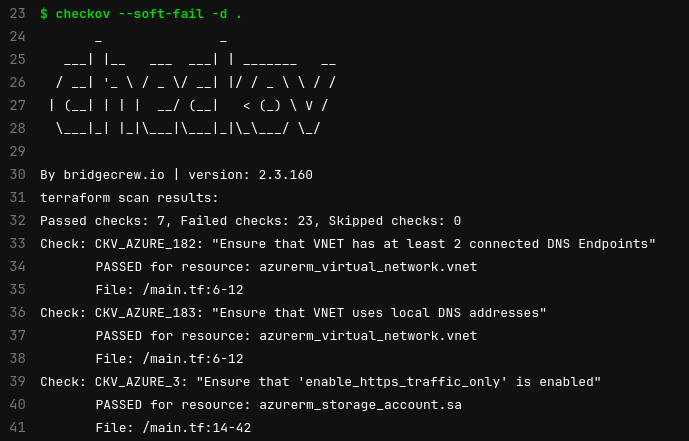
\includegraphics{../images/checkov-start.png}
            }
            \caption{Checkov analysis start and passed checks (O. Salvador, 2023)}
        \end{figure}

    For each of these problems that it finds, the culprit resource is shown, with a short description. Because some are false positives, and others are problemas which would require the reworking of my past report, which I consider beyond this one's scope, I've configured the jobs in which it's run to not fail the pipeline because of them. Checkov is a self-contained program, and has a Docker image with it preinstalled available. No permanent installation in the cluster has been necessary.
    \linebreak
    
        \begin{figure}[htb]
            \centering
            \resizebox{.9\linewidth}{!}{%
                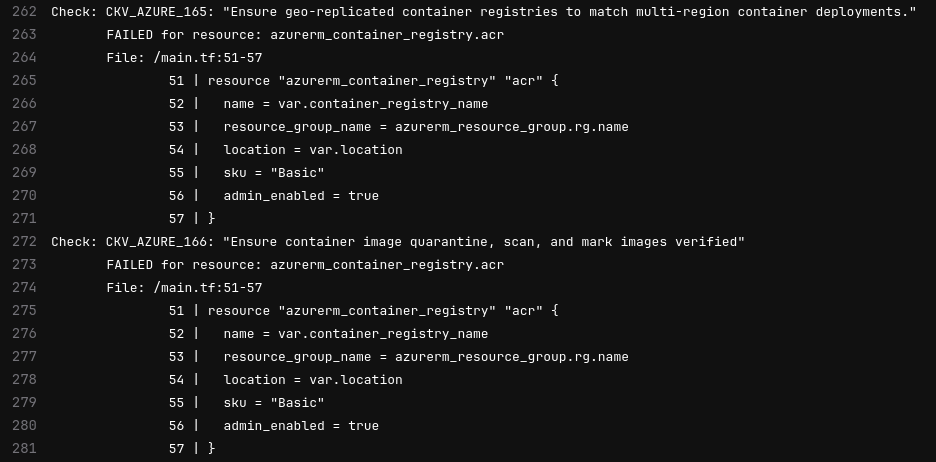
\includegraphics{../images/checkov-fails.png}
            }
            \caption{Checkov analysis failed security checks (O. Salvador, 2023)}
        \end{figure}

    The next two stages need the Azure CLI client, and Terraform. I have thus configured their jobs in the pipeline to seek out a runner that indicates their presence with tags. When \texttt{runner-setup.sh} was run on the VM, it registered the runner with those tags, so that it may now be found. If the script hasn't been executed, the runner no longer has connection to the cluster, or has been paused, plan and apply jobs that need those tags will be left as ``pending'', stuck until a runner with the tags is made available.
    \linebreak
    
        \begin{figure}[htb]
            \centering
            \resizebox{.7\linewidth}{!}{%
                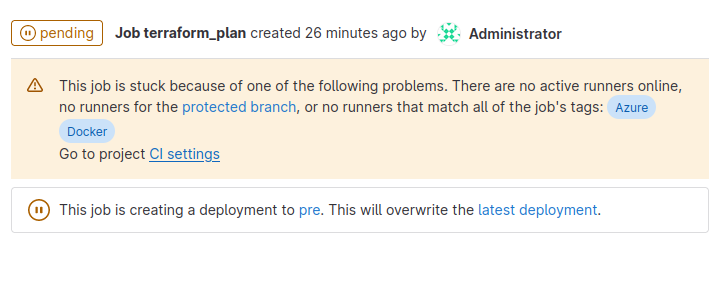
\includegraphics{../images/gitlab-pipeline-stuck2.png}
            }
            \caption{Terraform plan stuck due to no available runner with needed tags (O. Salvador, 2023)}
        \end{figure}








    \clearpage
    \subsection{Application pipelines}
    Pipelines for application source code projects can have up to four stages:
    
        \begin{itemize}
            \itemsep0em 
            \item Source code analysis: SCA and SAST are run automatically at the same time. 
    
            \item Build: build and push of the project's Docker image to the ACR
            
            \item Deploy: manual reset of the ACI, so that it starts again using the latest image (incurs downtime)

            \item Dynamic Application Security Testing with Arachni, manually triggered and only done in preproduction
    
        \end{itemize}

    \textit{\acrshort{owasp}} dependency-check is used for SCA. It's free and open source, doesn't need to be installed in the cluster, and was recommended by AWS in \cite{awsowasp}). Sonarqube, as described earlier, provides SAST. When jobs use specific images, these are run as ephemeral pods in the cluster's gitlab namespace. Since both SCA and SAST are part of the same stage, their pods get started at the same time.
    \linebreak
        
        \begin{figure}[htb]
            \centering
            \resizebox{.95\linewidth}{!}{%
                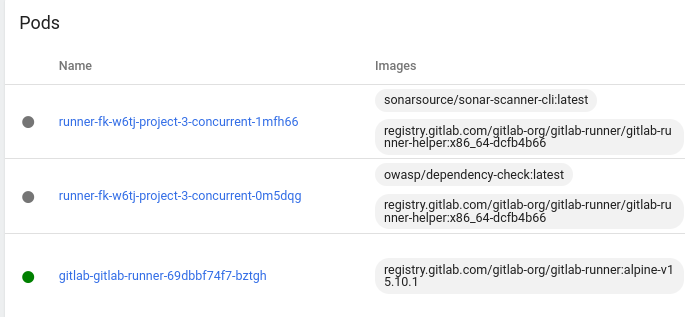
\includegraphics{../images/gitlab-runner-parallel-pods.png}
            }
            \caption{OWASP dependency check and Sonarscanner concurrently (O. Salvador, 2023)}
        \end{figure}

    The dependency-check script first downloads databases with known \textit{\acrshort{cve}} (\textit{\acrlong{cve}}, and then compares the code in the directory it's specified to scan with them, looking for versions of libraries that are known to be compromised. The SAST job uses Sonarqube's sonarscanner to connect with the server installed in the cluster.
    \linebreak


        \begin{figure}[htb]
            \centering
            \resizebox{.9\linewidth}{!}{%
                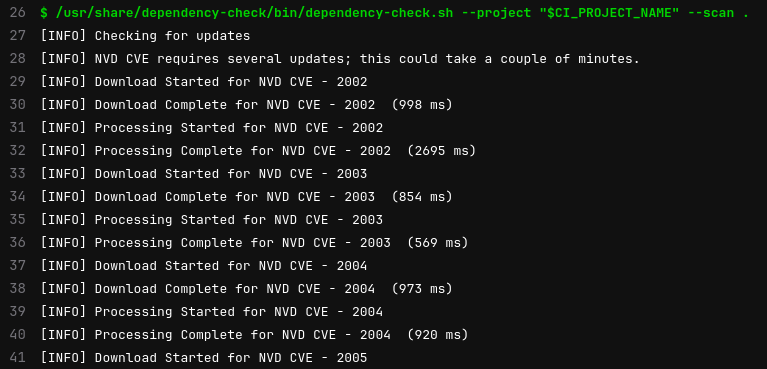
\includegraphics{../images/owasp-dep-check-start.png}
            }
            \caption{OWASP dependency-check start and download of CVEs (O. Salvador, 2023)}
        \end{figure}

        \begin{figure}[htb]
            \centering
            \resizebox{.9\linewidth}{!}{%
                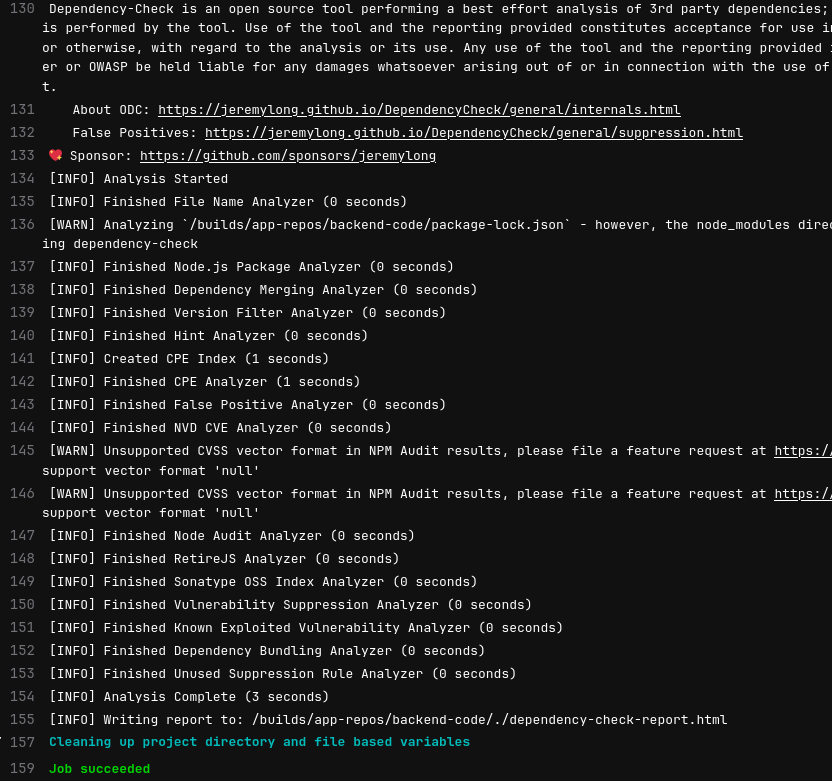
\includegraphics{../images/owasp-dep-check-finish2.png}
            }
            \caption{OWASP dependency-check finished (O. Salvador, 2023)}
        \end{figure}

    \clearpage
    Sonarqube's job uses the truststore (with the certificate) that was uploaded to all branches in all code projects. The two sonarqube variables that were created in the projects using Terraform are \texttt{\$SONAR\_KEYSTORE\_PW} and \texttt{\$SONAR\_TOKEN}. The first is used to decrypt the truststore and access the certificate in it, with which a secure tunnel can be established, even though the CA (which I trust) isn't signed by a known and popularly trusted CA. The second is used by \texttt{sonar-scanner}, to connect with the server and authenticate as a recognized and authorized user, so that the server accepts the scan request.
    \linebreak

        \begin{figure}[htb]
            \centering
            \resizebox{\linewidth}{!}{%
                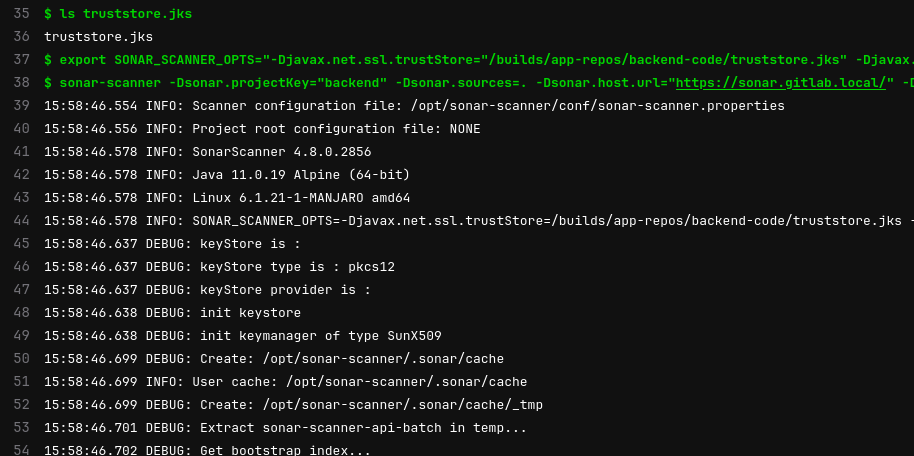
\includegraphics{../images/sonarqube-start.png}
            }
            \caption{Sonarqube start (O. Salvador, 2023)}
        \end{figure}

        \begin{figure}[htb]
            \centering
            \begin{subfigure}{.95\textwidth}
                \hspace{-5cm}
                \inputminted[fontsize=\scriptsize, firstline=1, lastline=2, linenos, frame=single, tabsize=1, breaklines]{bash}{../sonarqube-pipeline-commands.sh}
              \end{subfigure}
            \caption{Sonarqube pipeline job variables and \texttt{sonar-scanner} command with args, \texttt{frontend-code gitlab-ci.yml} (O. Salvador, 2023)}
        \end{figure}

    Sonarqube's scan results can be accessed in the instance's website (at \texttt{sonar.gitlab.local} as configured by my scripts). There, quality gates can be configured to consider the code valid or fail the pipeline. Because I have made no unit tests for the code of any project, a minimally stringent quality gate will fail the job, and with it, the stage and pipeline. Since I consider revisiting the previous report beyond this one's scope, I have made the job permissive to failure, so that the pipeline will not fail even if the job does.

        \begin{figure}[htb]
            \centering
            \resizebox{\linewidth}{!}{%
                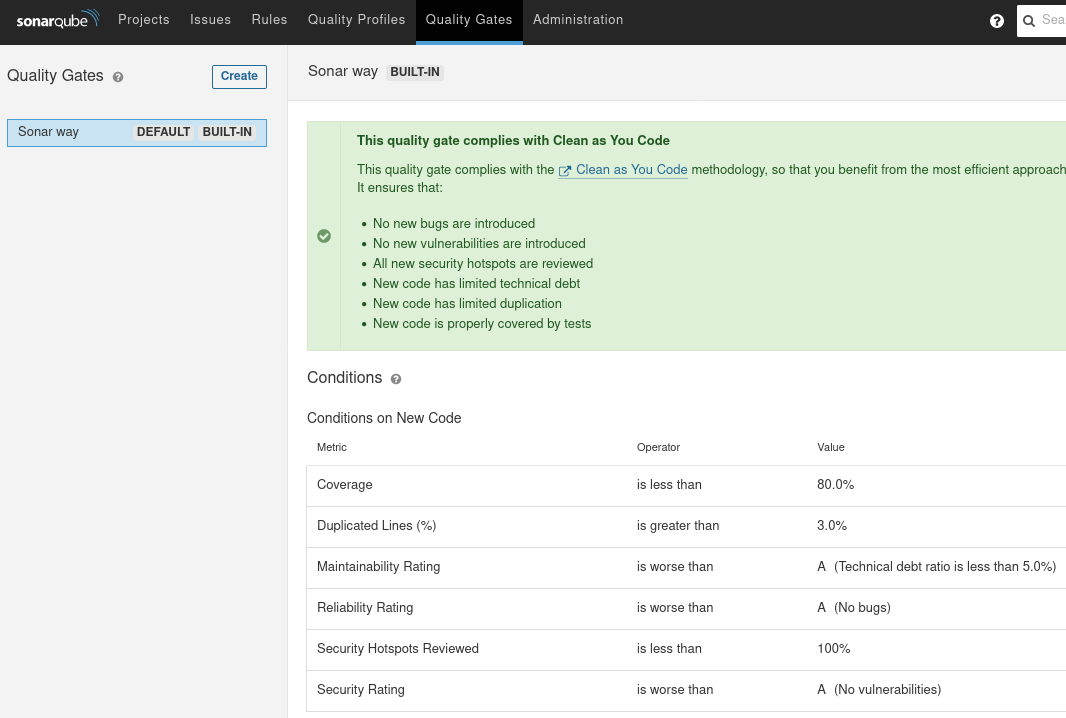
\includegraphics{../images/QualityGates2.png}
            }
            \caption{Built-in permissive Quality Gate (O. Salvador, 2023)}
        \end{figure}

        \begin{figure}[htb]
            \centering
            \resizebox{\linewidth}{!}{%
                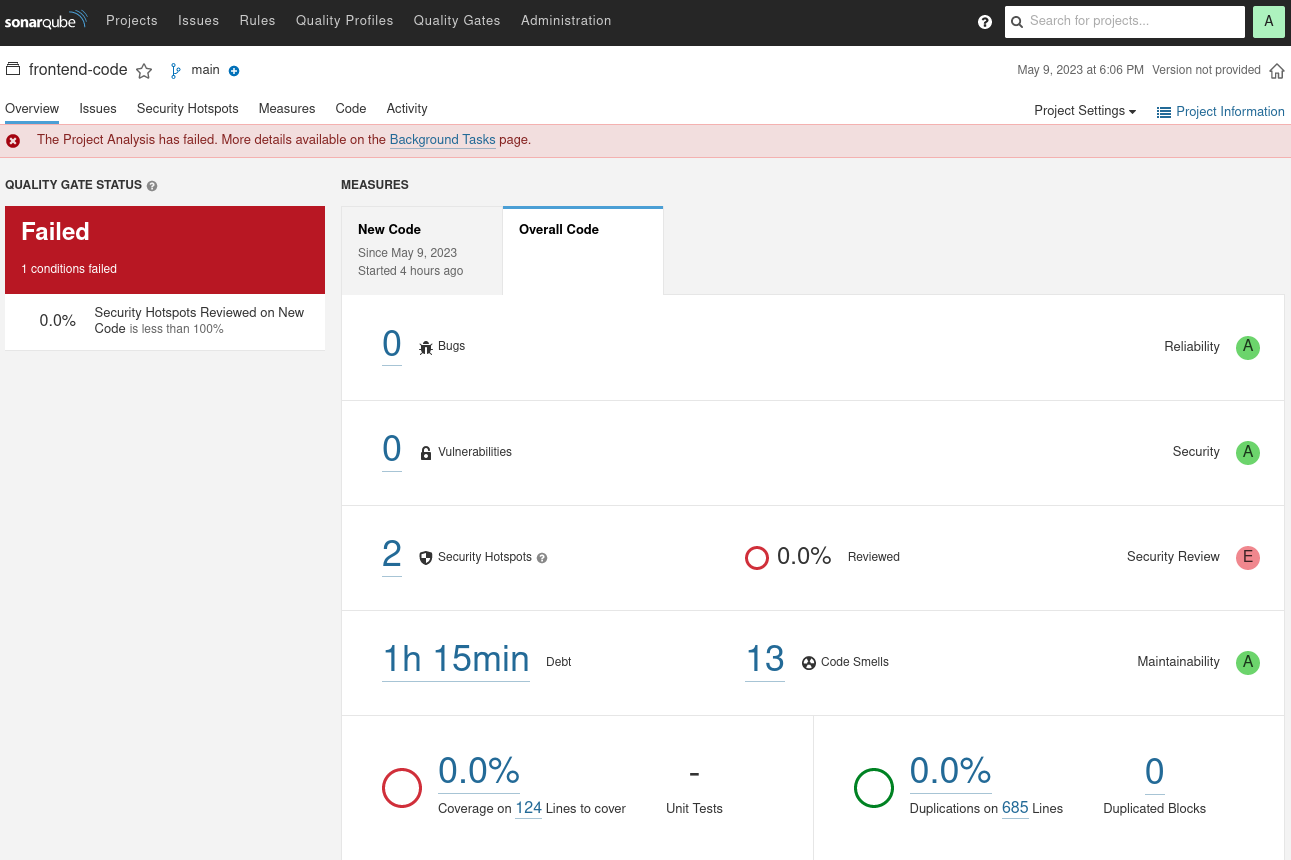
\includegraphics{../images/sonar-failed.png}
            }
            \caption{Scan of frontend-code failed due to poor security score (O. Salvador, 2023)}
        \end{figure}
        
    \clearpage
    
        \begin{figure}[htb]
            \centering
            \resizebox{\linewidth}{!}{%
                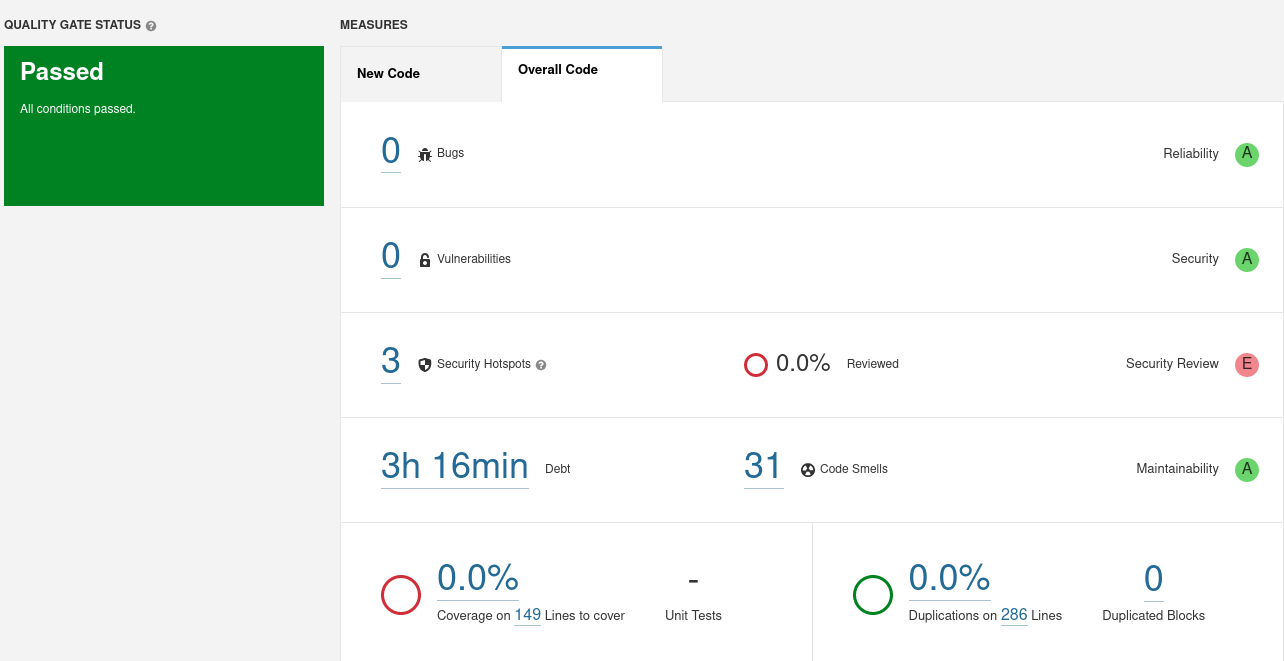
\includegraphics{../images/sonar-passed.png}
            }
            \caption{Scan of backend-code passed with permissive Quality Gate (O. Salvador, 2023)}
        \end{figure}

    Once the automatic analysis have been finished, the next stage, ``build'' starts. Although the GitLab runner in the cluster can build images, even though it's running in minikube with Docker as a driver for the nodes, by using Docker-in-Docker, since it later needs to be uploaded to the ACR (therefore use \texttt{az-cli}), I use the runner in the virtual machine. Only the runner in the VM meets the job's tags and can thus run it. 
    \linebreak

    The deployment of the images that have just been tagged as latest and made available in the ACR is manual. This means the pipeline does Continuous Delivery, but doesn't cross over to Continuous Deployment, which would be the automatic rollout of the changes. When it is triggered by a user, Terraform could have been used, and updated the entire ACI resource, or the same operation performed through \texttt{az-cli}, with \texttt{az container create} and the details of the already existing resource (to re-create it in-place). The latter is Microsoft's recommended method for updating ACIs (\cite{updateaci}). There is however a better method, that doesn't need to create the entire container instance again, and that is to reset it. When it's reset, the instance isn't removed, but the container itself is, and a new one is run from the image the instance is configured to use (\cite{aciaz}). By setting the image that has to be used as the project's latest corresponding one, when the previous stage pushed a new one, with the ``latest'' tag, that image became the one that would be used for new containers. Because ACIs don't have multiple containers running, any change of container implies downtime, but by just changing the container instead of the whole resource, the time required is shortened.
    \linebreak
            
    Only in the frontend's project, and just for the code deployed to preproduction (from the develop branch, not yet merged), another stage is available, with a manual trigger. The DAST job runs arachni against the FQDN of the preproduction frontend ACI. 
    \linebreak

    Arachni queries a large number of possible endpoints that might have been unintentionally left accessible, and shouldn't be, because of them posing a security risk. It also tries to find vulnerabilities in the webapp's code, like SQL injections or \textit{\acrlong{xss}} (\textit{\acrshort{xss}}). Like Checkov and OWASP dependency-check, it's free to use and open source, and doesn't need to be installed in the cluster, as a Docker image with it installed is available. This, as it did for the others without servers, makes it very easy to integrate into CI pipelines. The results of it's audits are available in the job's execution log.
    \linebreak
    
        \begin{figure}[htb]
            \centering
            \resizebox{.88\linewidth}{!}{%
                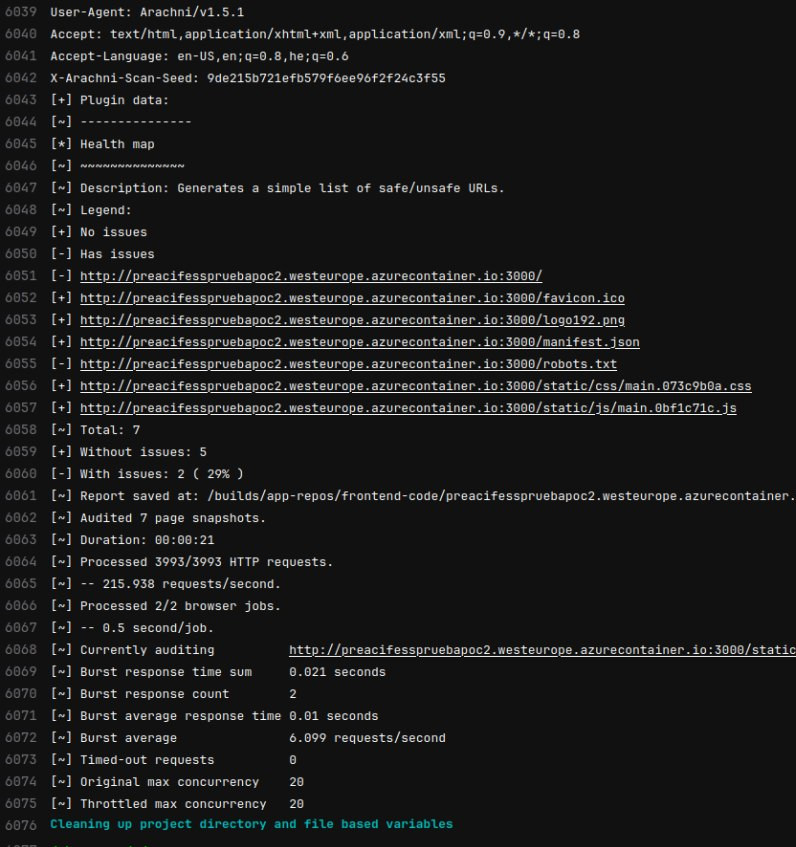
\includegraphics{../images/arachni-crop.jpg}
            }
            \caption{Result of Arachni DAST scan on the frontend (O. Salvador, 2023)}
        \end{figure}
























\clearpage
\section{Conclusion}
This project has helped me deepen my understanding of DevOps and DevSecOps, and clear some misconceptions I previously had. Having the cluster, with all it's elements setup wouldn't have helped me develop the previous report's project quicker. Most of the work would have been the same. But some features could have been tested from the beginning, and had I been working with the preproduction environment I now have available, I wouldn't have had to first make a local system, and then look for ways to make it work in the cloud. It would have been possible to start developing against the same cloud components I would use in production from the start. The last month of the project in particular, was spent trying to work around decisions made without knowledge of the intricacies the system would end up having. What I can confidently say however, is the code I released the last semester would have been of a higher quality, with security recommendations from all the tools that are now integrated and easily used, upon every commit made.
\linebreak

Developing this system has made me work with Bash and Terraform a lot, and Terraform at the same time as I used it at EVO Banco, with my work at home and at the office feeding into each other. This has been very valuable, and I now consider myself well-versed with the tool. I've also had to work with Kubernetes, which I've barely had to do at work, and with encrypted HTTP, which I haven't done at any other point. The setup and use of the systems security analysis tools and the work with certificates and HTTPS have given me an on-hands appreciation of the implications and duties maintaining cybersecurity entails. It cannot be an afterthought, and has few shortcuts.
\linebreak

I leave this course having had to integrate many different tools into a coherent and useful system, which has not been an easy feat to achieve. This experience, along with what I've learned at TechSociety and EVO Banco have given me a more holistic perspective, along with comprehensive technical know-how of ``DevOps''. It's not a \textit{buzzword}, but a set of practices with value for large projects, and that takes considerable work to get working. There's no way this work could have been fit into the previous course's timetable.
\linebreak


\clearpage
\section{Future lines of work}
During the development of this project, I've had to leave out several desirable pieces of work, that couldn't be fit into it's finite development time. In the same way this project followed up one the previous' outlined recommendation for a Software Life Cycle Development DevOps system, and then expanded upon it adding security measures, upgrading it into a fully-fledged DevSecOps system, newly found points of improvement are left to a future effort. These are:
\linebreak

    \begin{itemize}
        \itemsep0em 
        \item Migration of the backend and frontend servers from Azure Container Instances into another, separate, Kubernetes cluster, for the application's components. This would allow multiple instances of each server to exist, and for their images to be swapped out without downtime. Green/blue, or canary deployments (among other possibilities) of the code would be possible, slowly re-routing customer traffic from pods with the old code to pods with the latest changes. This would improve the application's availability and be more inline with \textit{\acrshort{ha}} practices. The lack of implied downtime could also be used for continuous deployment, which I shied away from because of. 
        \linebreak

        \item Switch from continuous delivery to completely continuous deployment, once the previous line of work has been exhausted and it's viable to do so.
        \linebreak
        
        \item Rework of the application's code and IaC following the recommendations the DevSecOps components in the pipelines outline. It would have been prohibitive to also return to the code while developing this project's, but now that it's finished, it only follows to make use of it's functionalities.
        \linebreak

        \item Comparison of the real performance and usefulness of different tools for the different security tests, comparing the offerings of providers such as Lacework or Snyk with the current system.
        \linebreak
        
        \item Use of a certificate signed by an trusted third party like Let's Encrypt, instead of the certificate I created on my own.

        
        
    \end{itemize}






    
% en la seccion de evo decir que usan ITIL, aunque tristemente no lo he dado en la uni



\clearpage
\appendix
\section{Repository and use}
\label{anexo:grafico}
This project's source code is openly available in my GitHub at \cite{misgit2}. The final release before this report's due date is available at \texttt{\url{https://github.com/oscarsalvador/NEB-practica-empresa-2/releases/tag/v1}}. It's comprised of the Bash scripts described in this report. It requires a host with at least 32 gigabytes of RAM, and eight to twelve cores. The machine needs to have Docker, Helm, Minikube, and Kubectl installed. The three latter can be downloaded and made available to the system with the included \texttt{download.sh} script. Another machine is also required, and it needs to have access to the one in which \texttt{launch.sh} is triggered. In my tests I used a VirtualBox virtual machine, but the same host could also be used. This machine needs to have Azure CLI, Docker, and Terraform installed. Additionally, the scripts expect \texttt{az-cli} to be already logged into.
\linebreak

Executing \texttt{launch.sh} will make changes to \texttt{/etc/hosts}, appending a line with the subdomains that will be used. It will also result in several docker images being downloaded to the local registry.





\end{flushleft}

\clearpage
\printbibliography[heading=bibintoc]

\end{document}
